\section{Diagramas de Sequência}

Nesta seção, são apresentados os diagramas de sequência que descrevem o comportamento dinâmico do sistema frente às interações dos usuários com as principais funcionalidades.

\subsection{Diagrama de Sequência – Criação de Novo Usuário}

A Figura~\ref{fig:diagrama-criacao-usuario} ilustra o fluxo realizado pelo administrador ao criar um novo usuário no sistema. Esse processo envolve o acesso ao módulo de gestão de usuários, abertura do formulário de cadastro, preenchimento dos campos necessários, validação dos dados e envio para o backend.

\begin{figure}[H]
    \centering
    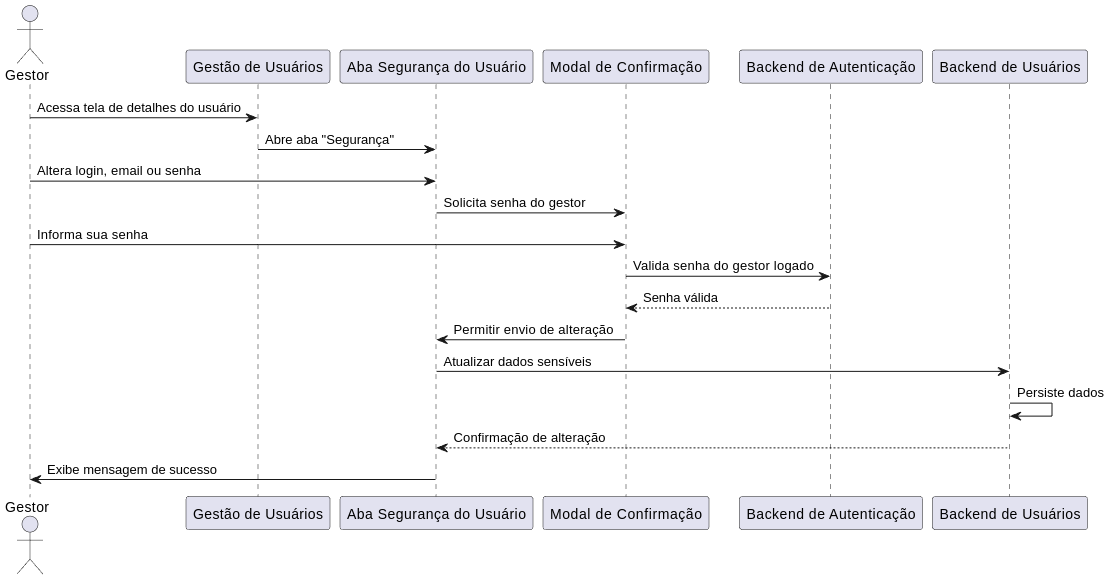
\includegraphics[width=0.9\textwidth]{images/diagramasdesequencias/usercreate.png}
    \caption{Diagrama de sequência para criação de novo usuário}
    \label{fig:diagrama-criacao-usuario}
\end{figure}

O fluxo se inicia quando o administrador clica no botão “+ Novo Usuário”. O sistema exibe o formulário de cadastro, onde o administrador preenche os dados como nome, e-mail, senha e papel do usuário. O formulário aciona a validação dos campos obrigatórios. Com os dados validados, a informação é enviada ao backend, que cria o novo registro no banco de dados. Em seguida, o sistema exibe uma mensagem de sucesso e atualiza a lista de usuários visível para o administrador.

\subsection{Diagrama de Sequência – Visualização e Edição de Permissões}

A Figura~\ref{fig:diagrama-permissoes} ilustra o fluxo realizado pelo administrador para visualizar e editar as permissões de um usuário. O processo envolve a seleção do usuário, acesso à aba de permissões e modificação das permissões conforme necessário.

\begin{figure}[H]
    \centering
    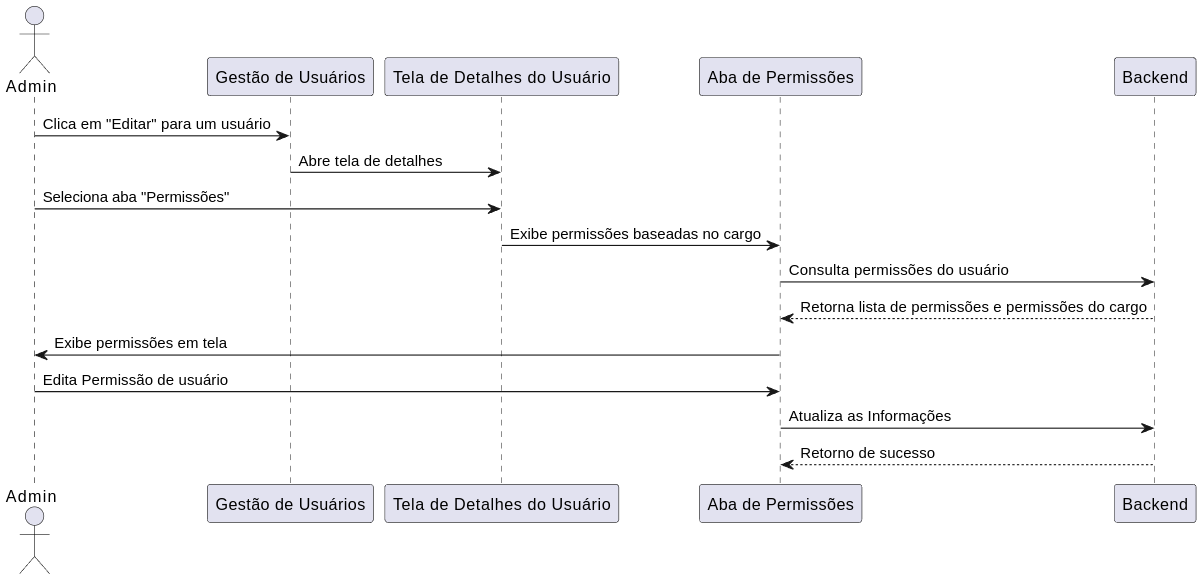
\includegraphics[width=0.9\textwidth]{images/diagramasdesequencias/userEditPermissions.png}
    \caption{Diagrama de sequência para visualização e edição de permissões de usuário}
    \label{fig:diagrama-permissoes}
\end{figure}

\subsection{Diagrama de Sequência – Edição de Informações do Usuário}

A Figura~\ref{fig:diagrama-edicao-usuario} ilustra o fluxo realizado pelo administrador ao editar informações cadastrais de um usuário. Esse processo permite a atualização de dados como nome, cidade, data de nascimento e cargo.

\begin{figure}[H]
    \centering
    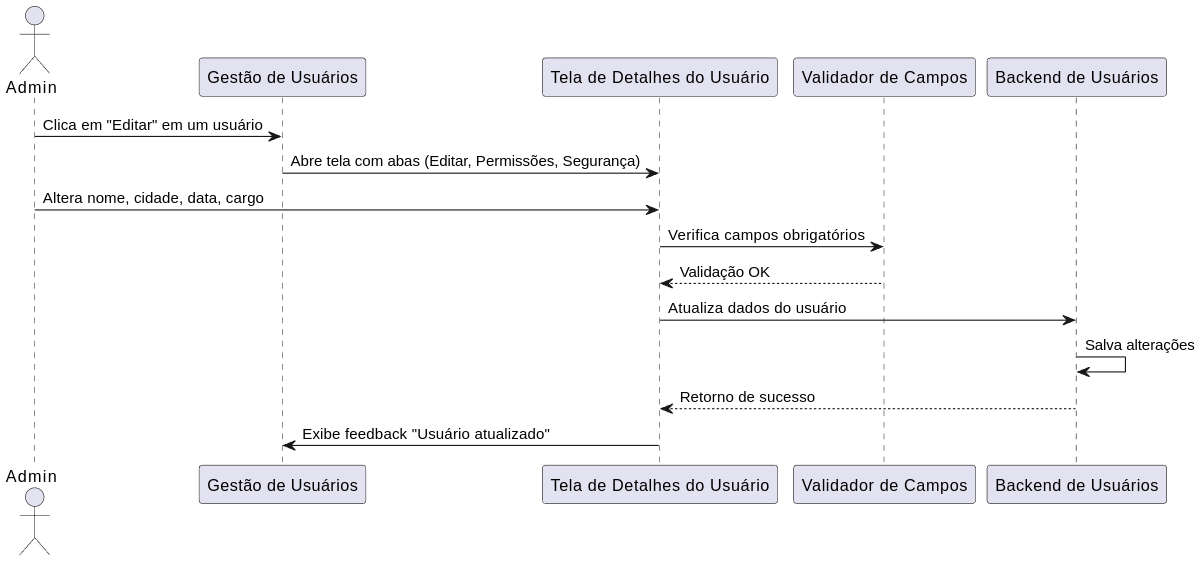
\includegraphics[width=0.9\textwidth]{images/diagramasdesequencias/userEdit.png}
    \caption{Diagrama de sequência para edição de informações do usuário}
    \label{fig:diagrama-edicao-usuario}
\end{figure}

O fluxo se inicia quando o administrador acessa o módulo de gestão de usuários e clica na opção “Editar” para um usuário específico. A tela de detalhes do usuário é carregada com múltiplas abas, sendo selecionada a aba de edição. Após realizar as alterações nos campos, o sistema valida os dados obrigatórios. Com a validação concluída, os dados são enviados ao backend para atualização no banco de dados. Por fim, uma mensagem de sucesso é exibida ao administrador confirmando a atualização.

\subsection{Diagrama de Sequência – Edição de Dados Sensíveis com Confirmação}

A Figura~\ref{fig:diagrama-dados-sensiveis} apresenta o fluxo que ocorre quando o gestor edita dados sensíveis de um usuário, como login, e-mail ou senha. Este processo exige uma etapa adicional de autenticação para garantir a segurança da operação.

\begin{figure}[H]
    \centering
    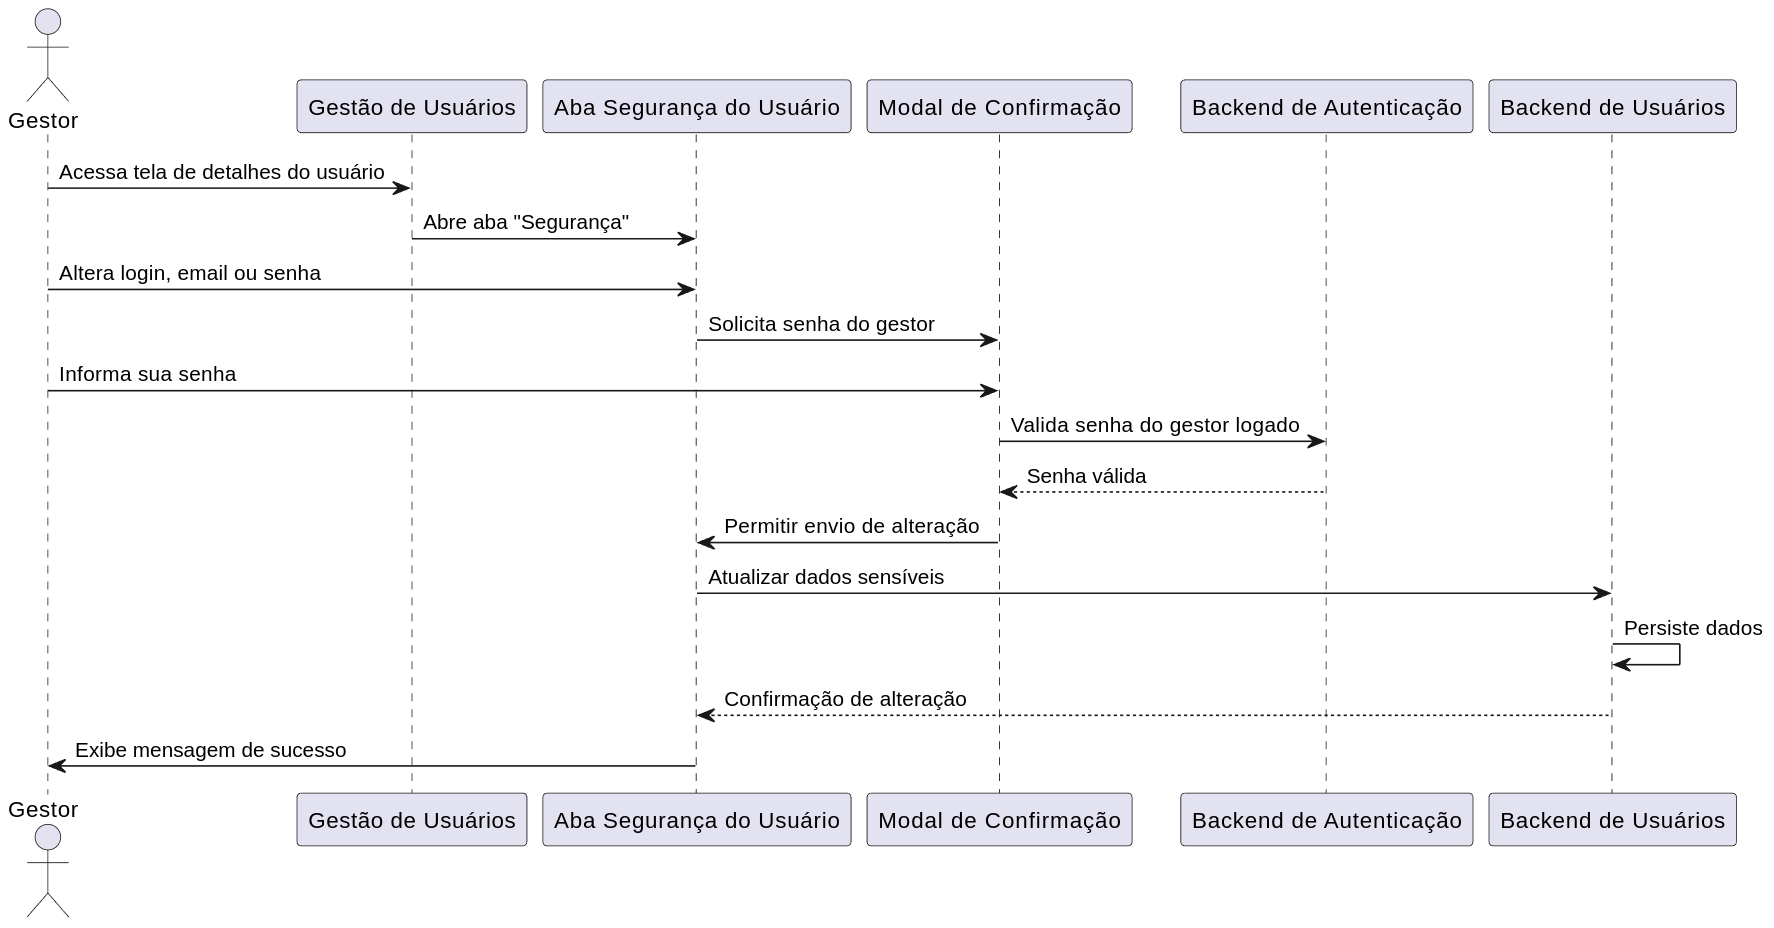
\includegraphics[width=0.9\textwidth]{images/diagramasdesequencias/userCredentials.png}
    \caption{Diagrama de sequência para edição de dados sensíveis com confirmação}
    \label{fig:diagrama-dados-sensiveis}
\end{figure}

O fluxo inicia-se com o gestor acessando a tela de detalhes do usuário e navegando até a aba “Segurança”. Ao tentar alterar dados sensíveis, como login, e-mail ou senha, o sistema exibe um modal solicitando a senha do gestor para confirmar a ação. Após a senha ser informada, ela é validada pelo backend de autenticação. Com a validação bem-sucedida, o sistema autoriza a atualização, que é enviada ao backend de usuários. Após a persistência dos dados no banco, o sistema exibe uma mensagem de confirmação ao gestor.

\subsection{Diagrama de Sequência – Login de Usuário}

A Figura~\ref{fig:normalLogin} apresenta o fluxo completo do processo de autenticação de um usuário no sistema. Esse processo envolve a verificação das credenciais, a inicialização da sessão e a exibição da interface conforme o papel atribuído ao usuário.

\begin{figure}[H]
    \centering
    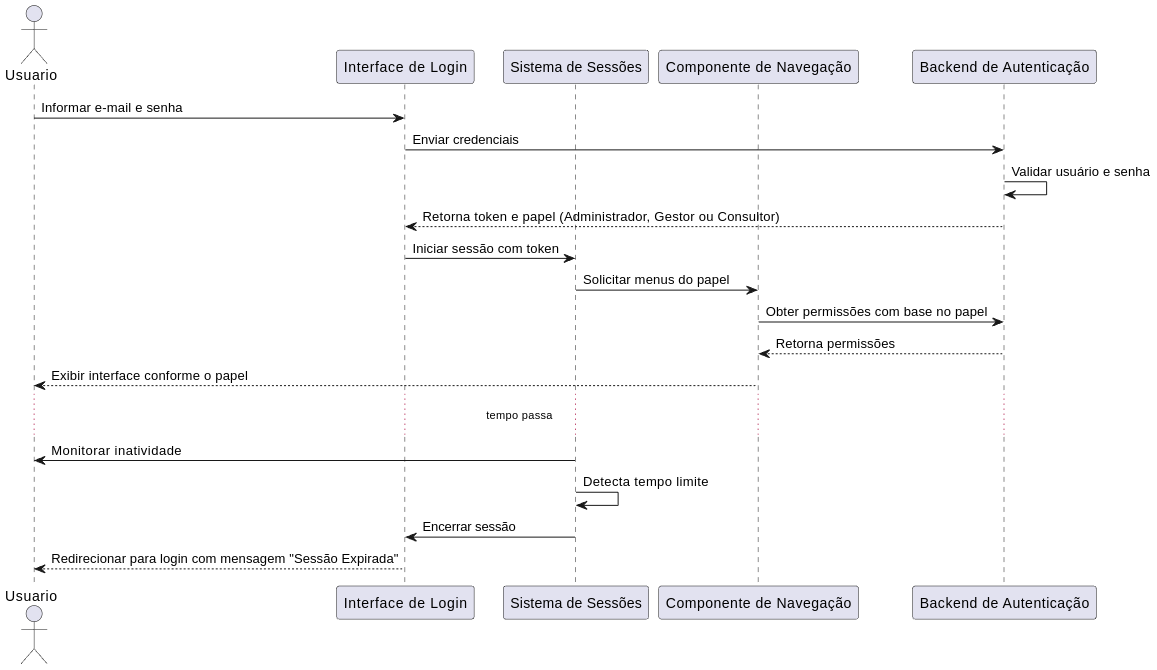
\includegraphics[width=0.9\textwidth]{images/diagramasdesequencias/normalLogin.png}
    \caption{Diagrama de sequência para login de usuário}
    \label{fig:normalLogin}
\end{figure}

O fluxo inicia-se quando o usuário informa seu e-mail e senha na interface de login. As credenciais são enviadas ao backend de autenticação, que realiza a validação e retorna um token e o papel do usuário (Administrador, Gestor ou Consultor). A sessão é iniciada com base nesse token, e a interface de navegação solicita ao backend as permissões correspondentes ao papel. Com base nas permissões, a interface adaptada é exibida ao usuário.

Após o login, o sistema monitora a atividade do usuário. Caso ocorra inatividade por tempo prolongado, a sessão é finalizada automaticamente, redirecionando o usuário à tela de login com a mensagem "Sessão Expirada".

\subsection{Diagrama de Sequência – Cadastro de Retiro}

A Figura~\ref{fig:retreatCreate} apresenta o fluxo realizado pelo gestor ao cadastrar um novo retiro no sistema. Esse processo envolve a abertura do formulário, preenchimento das informações principais, validação dos campos obrigatórios e comunicação com o backend para persistência dos dados.

\begin{figure}[H]
    \centering
    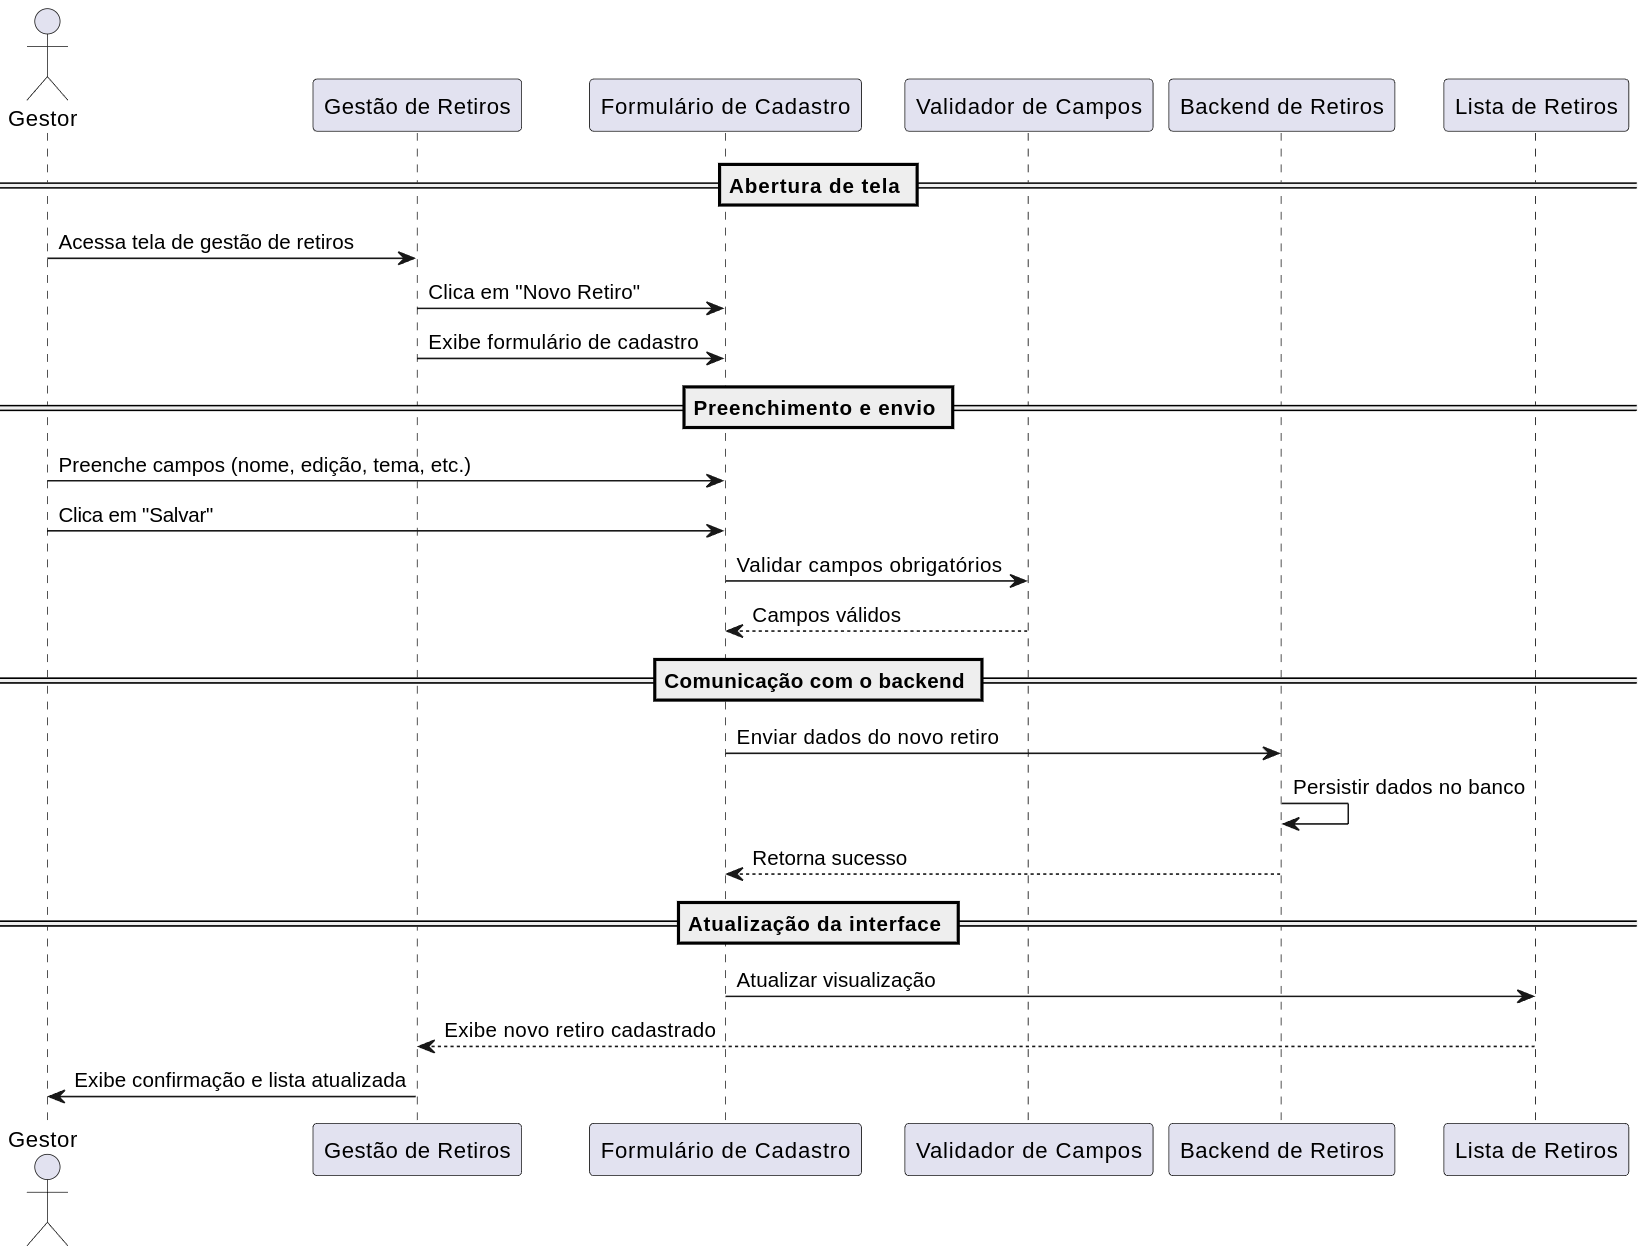
\includegraphics[width=0.9\textwidth]{images/diagramasdesequencias/retreatCreate.png}
    \caption{Diagrama de sequência para cadastro de retiro}
    \label{fig:retreatCreate}
\end{figure}

Inicialmente, o gestor acessa a tela de gestão de retiros e clica na opção “Novo Retiro”, o que aciona a exibição do formulário de cadastro. Após preencher os campos como nome, edição e tema, o gestor clica em “Salvar”. Os dados são validados e, se estiverem corretos, enviados ao backend para persistência. Ao final do processo, a lista de retiros é atualizada e o sistema exibe uma confirmação do cadastro.

\subsection{Diagrama de Sequência – Inativação de Retiro}

A Figura~\ref{fig:retreatInativation} apresenta o fluxo realizado pelo gestor para inativar um retiro previamente cadastrado. O processo envolve a seleção do retiro, confirmação da ação e atualização do status na interface.

\begin{figure}[H]
    \centering
    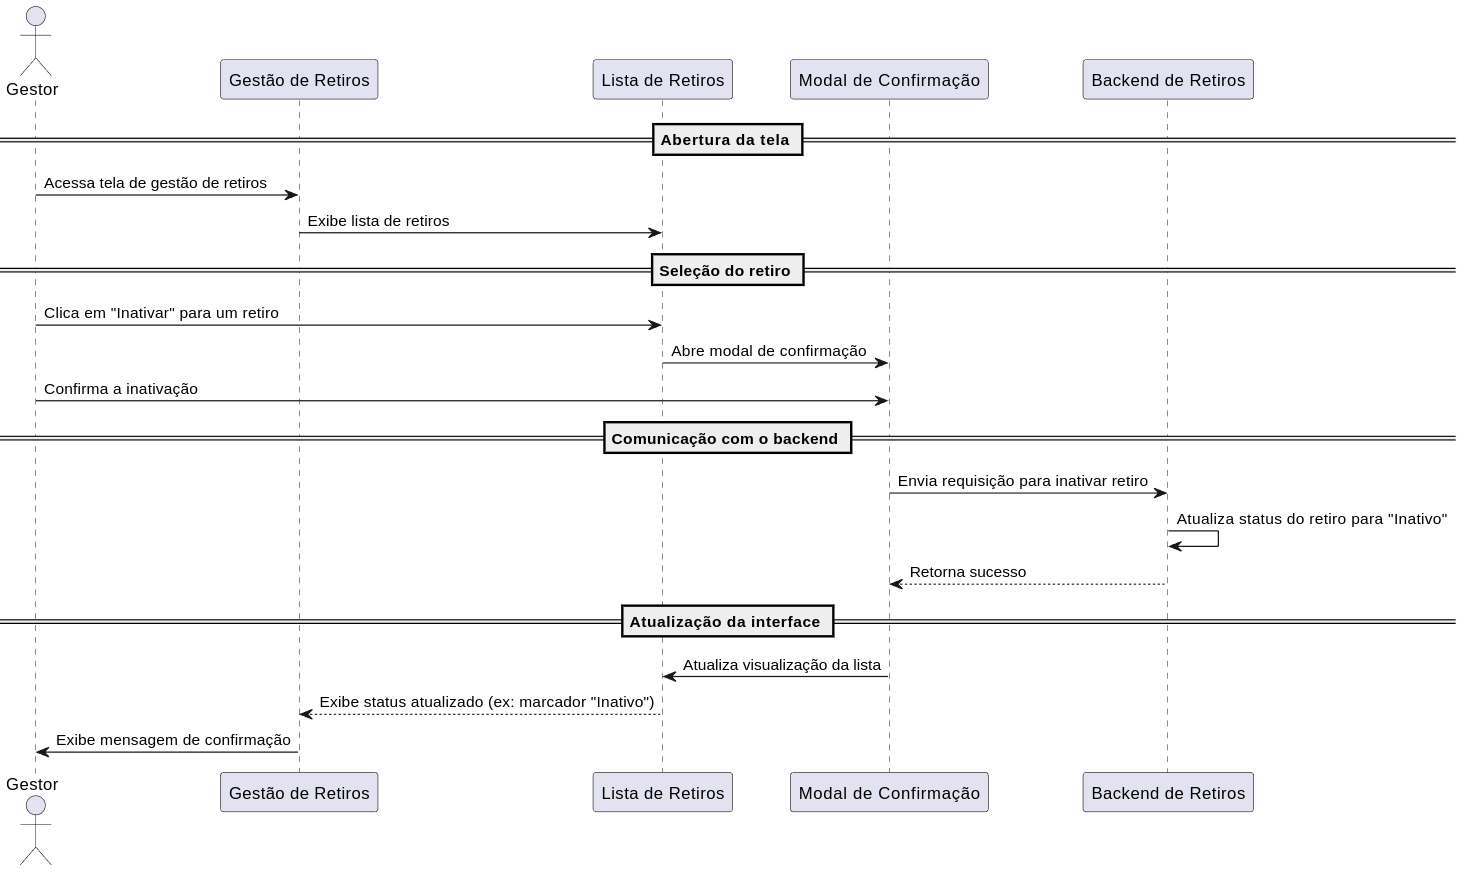
\includegraphics[width=0.9\textwidth]{images/diagramasdesequencias/retreatInativation.png}
    \caption{Diagrama de sequência para inativação de retiro}
    \label{fig:retreatInativation}
\end{figure}

O fluxo inicia com o gestor acessando a tela de gestão de retiros, onde é exibida a lista de eventos. Ao clicar em “Inativar” para um retiro específico, um modal de confirmação é apresentado. Após a confirmação, a requisição é enviada ao backend, que atualiza o status do retiro para “Inativo”. O sistema então retorna uma confirmação, atualiza a interface com um marcador indicativo e exibe uma mensagem de sucesso ao gestor.

\subsection{Diagrama de Sequência – Gerador de Formulário Personalizado}

A Figura~\ref{fig:retreatFormCreate} apresenta o fluxo realizado pelo gestor ao acessar e personalizar os formulários vinculados a um retiro. O sistema permite criar e editar formulários específicos tanto para os participantes quanto para as equipes de serviço, de forma modular.

\begin{figure}[H]
    \centering
    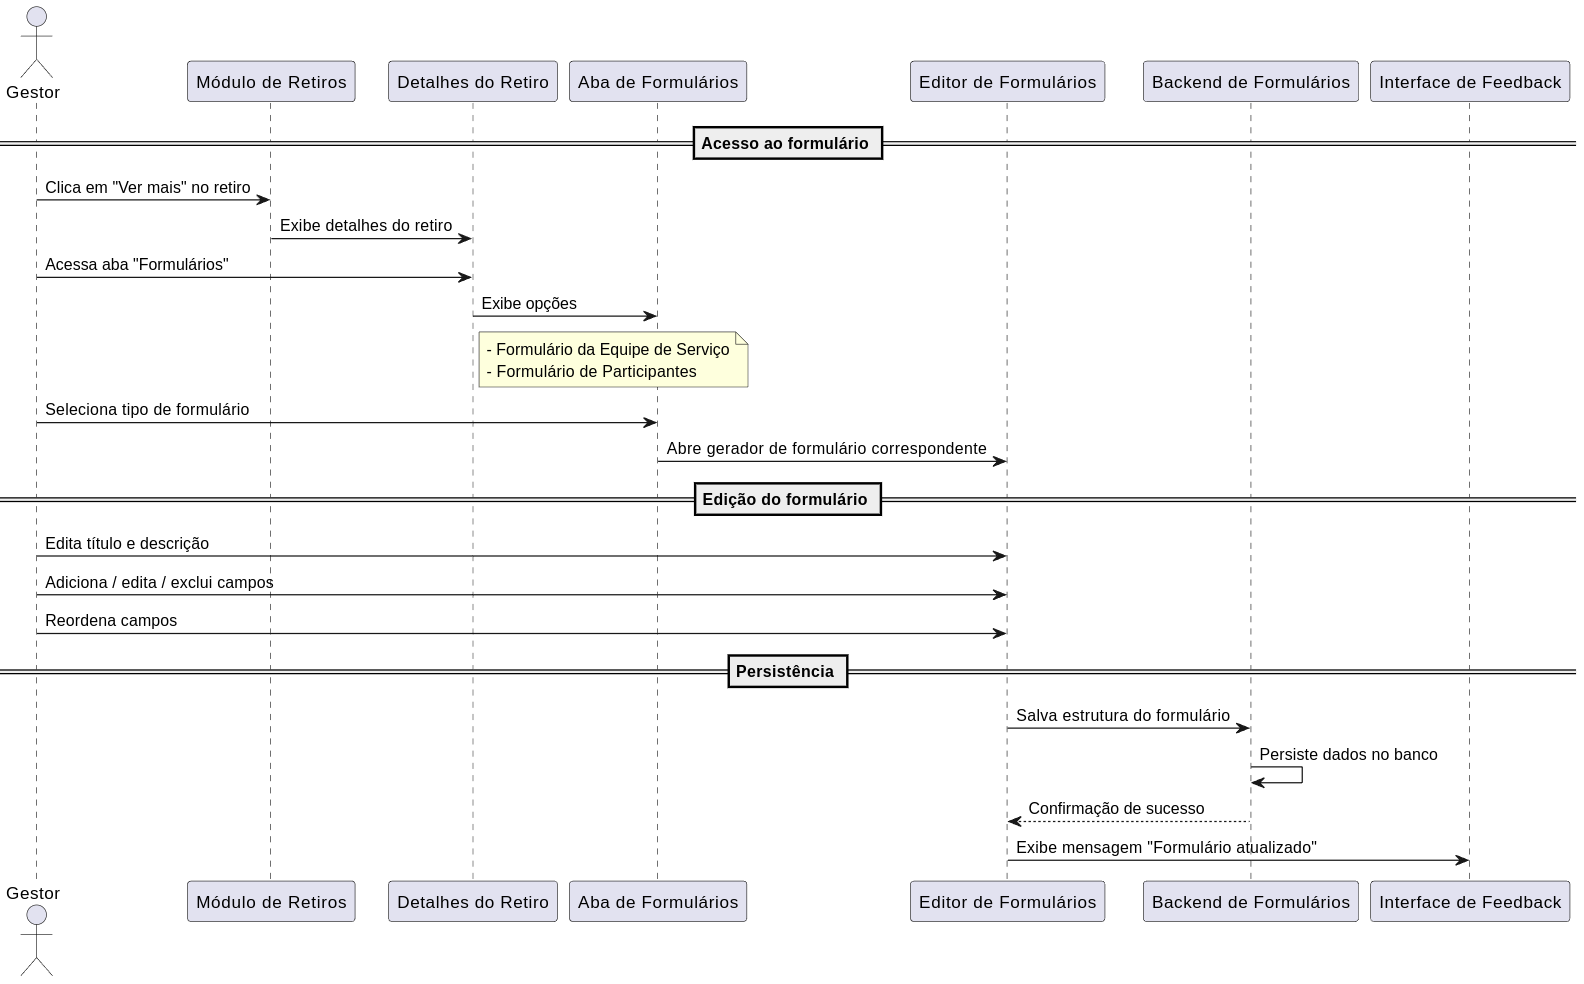
\includegraphics[width=0.9\textwidth]{images/diagramasdesequencias/retreatFormCreate.png}
    \caption{Diagrama de sequência para criação de formulário personalizado para um retiro}
    \label{fig:retreatFormCreate}
\end{figure}

O processo tem início quando o gestor acessa a área de detalhes de um retiro e seleciona a aba “Formulários”. Nessa aba, é possível escolher entre diferentes tipos de formulário. Como cada retiro tem 2 formulários(Participantes e equipe de serviço), você decide para qual grupo você irá editar, ao selecionar um deles, o sistema abre o editor correspondente. No editor, o gestor pode modificar o título, a descrição, adicionar ou remover campos e reordená-los conforme necessário. Ao salvar, o editor envia os dados ao backend, que persiste a estrutura do formulário e retorna uma confirmação. Por fim, uma mensagem é exibida ao gestor informando que a atualização foi bem-sucedida.

\subsection{Diagrama de Sequência – Inscrição Manual via Sistema}

A Figura~\ref{fig:manualParticipantInscription} descreve o fluxo completo para realização de inscrições manuais pelo gestor dentro do sistema, contemplando tanto o cadastro individual quanto a importação em lote via arquivo `.csv`.

\begin{figure}[H]
    \centering
    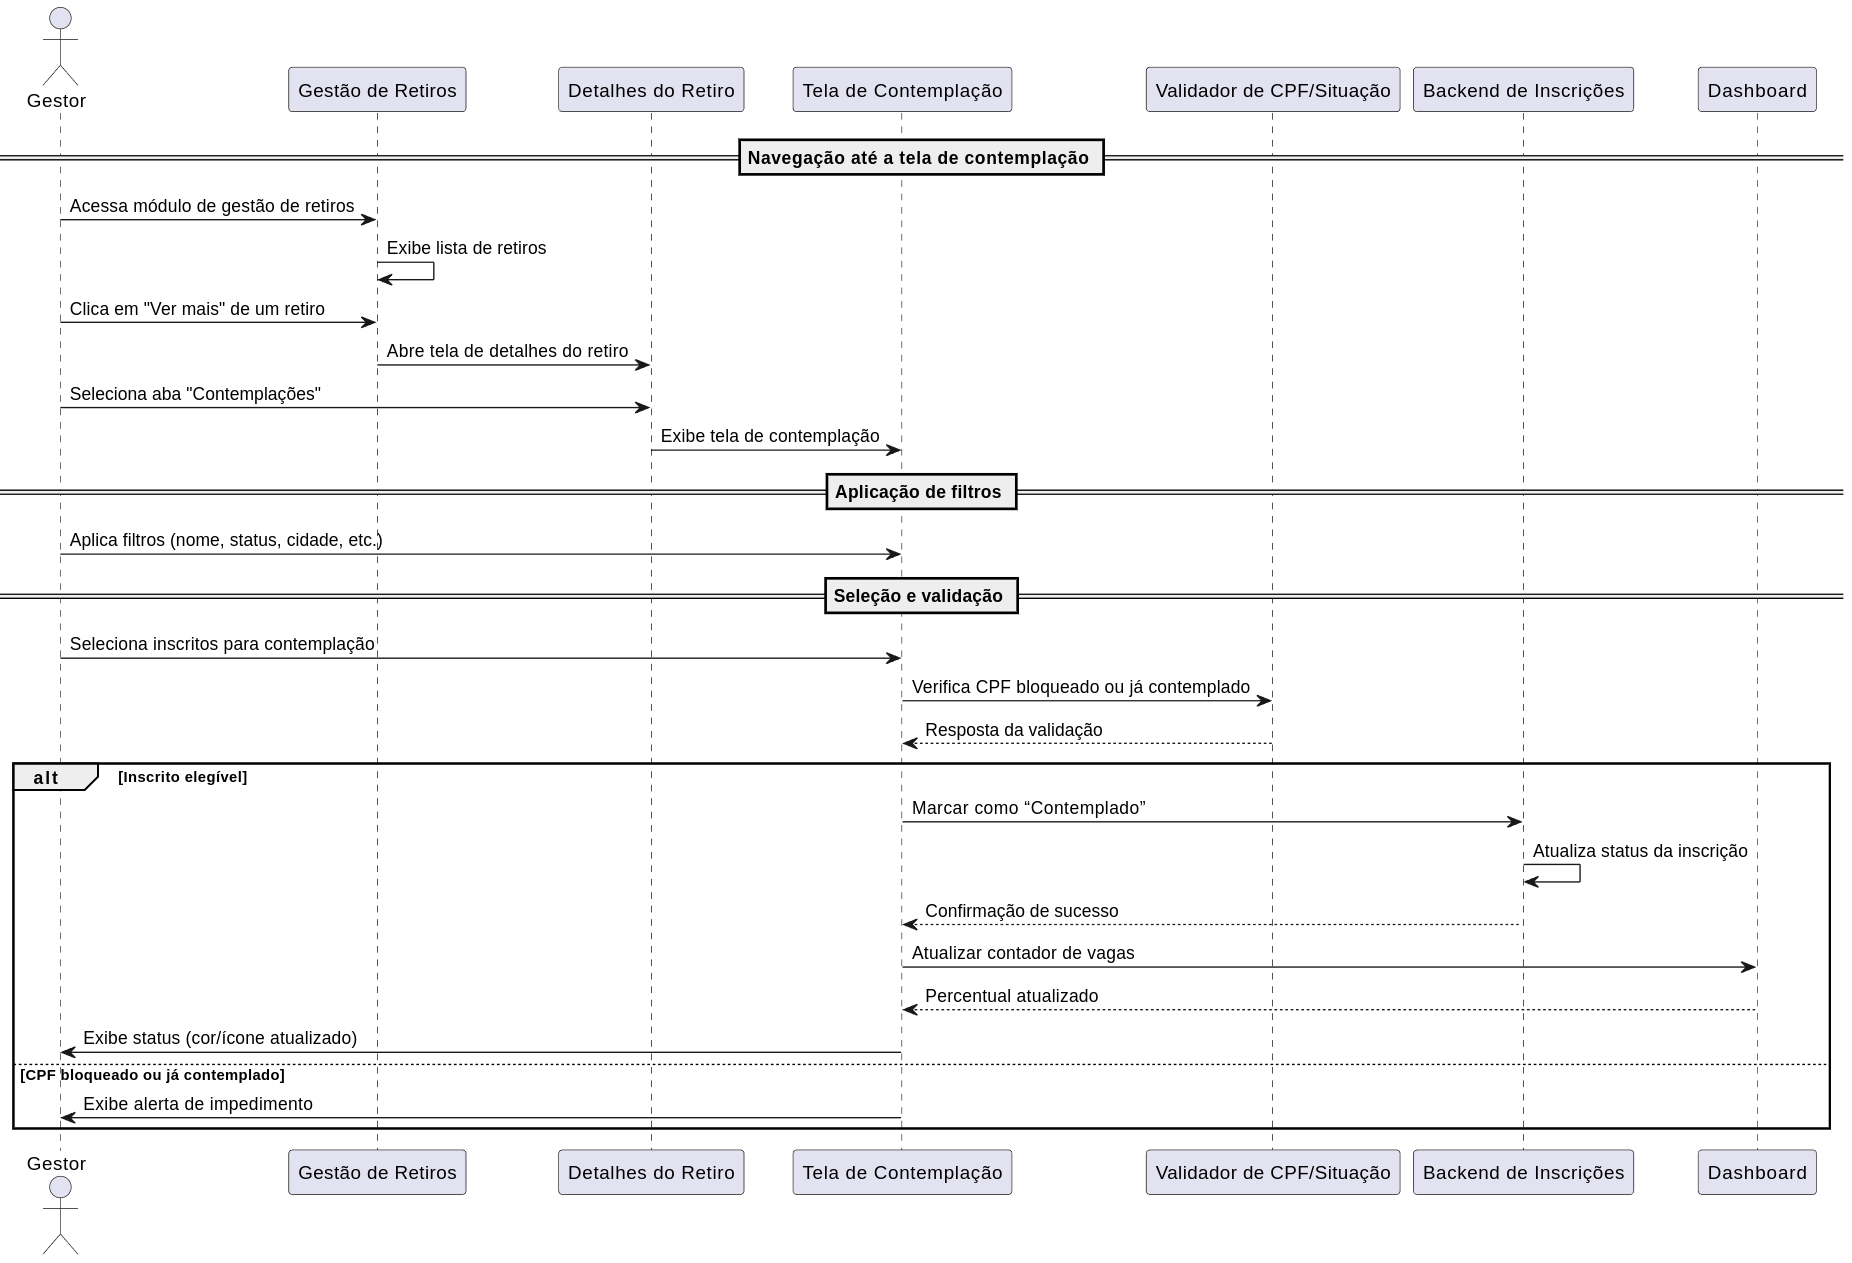
\includegraphics[width=0.9\textwidth]{images/diagramasdesequencias/manualParticipantSubscription.png}
    \caption{Diagrama de sequência para inscrição manual de participantes}
    \label{fig:manualParticipantInscription}
\end{figure}

O fluxo tem início com o gestor acessando o módulo de inscrições dentro do retiro selecionado. Ao optar por realizar o cadastro manual, o sistema apresenta o formulário interno com os mesmos campos do formulário público. Após o preenchimento, os dados são validados quanto à obrigatoriedade e à situação do CPF. Caso o CPF esteja bloqueado, o sistema retorna uma mensagem de erro. Se os dados forem válidos, a inscrição é armazenada e o gestor recebe a confirmação de sucesso.

Na alternativa de importação, o gestor seleciona um arquivo `.csv`. O sistema valida todas as linhas e separa aquelas com erro das válidas. As inscrições corretas são processadas em lote pelo backend, e ao final, é exibido um resumo com o número de registros bem-sucedidos e rejeitados.

\subsection{Diagrama de Sequência – Pagamento Manual via WhatsApp}

A Figura~\ref{fig:participantPayment} descreve o fluxo realizado pelo gestor ao confirmar manualmente o pagamento de um participante que enviou comprovante via WhatsApp. Esse processo inclui a navegação até o inscrito, edição do status de pagamento e envio do comprovante.

\begin{figure}[H]
    \centering
    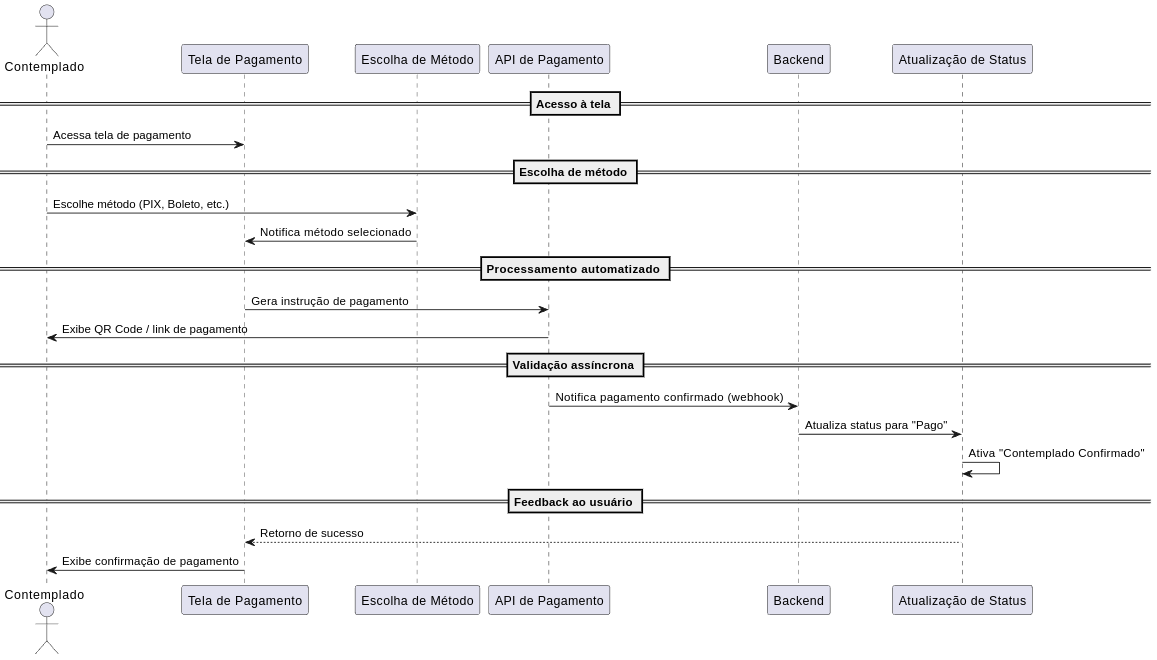
\includegraphics[width=0.9\textwidth]{images/diagramasdesequencias/participantPayment.png}
    \caption{Diagrama de sequência para confirmação manual de pagamento via WhatsApp}
    \label{fig:participantPayment}
\end{figure}

O fluxo se inicia com o gestor acessando os detalhes de um retiro e navegando até a aba “Contemplados”. Após localizar o inscrito, o gestor realiza um clique com o botão direito para abrir o menu de contexto e seleciona a opção “Editar Pagamento”. Um modal é exibido, permitindo ao gestor alterar o status de pagamento de “Pendente” para “Pago” e fazer upload do comprovante recebido (imagem ou PDF).

O sistema realiza a validação do arquivo enviado quanto ao tipo e tamanho. Caso esteja válido, a informação é enviada ao backend, que armazena o comprovante e atualiza o status do participante. Por fim, uma mensagem de confirmação é exibida e a lista de contemplados é atualizada com o novo status.

\subsection{Diagrama de Sequência – Envio de Mensagem de Contemplação}

\subsection{Diagrama de Sequência – Contemplação de Participantes}

A Figura~\ref{fig:participantContemplation} apresenta o fluxo realizado pelo gestor ao contemplar participantes inscritos em um retiro, incluindo etapas de filtro, validação de elegibilidade e atualização de status e indicadores.

\begin{figure}[H]
    \centering
    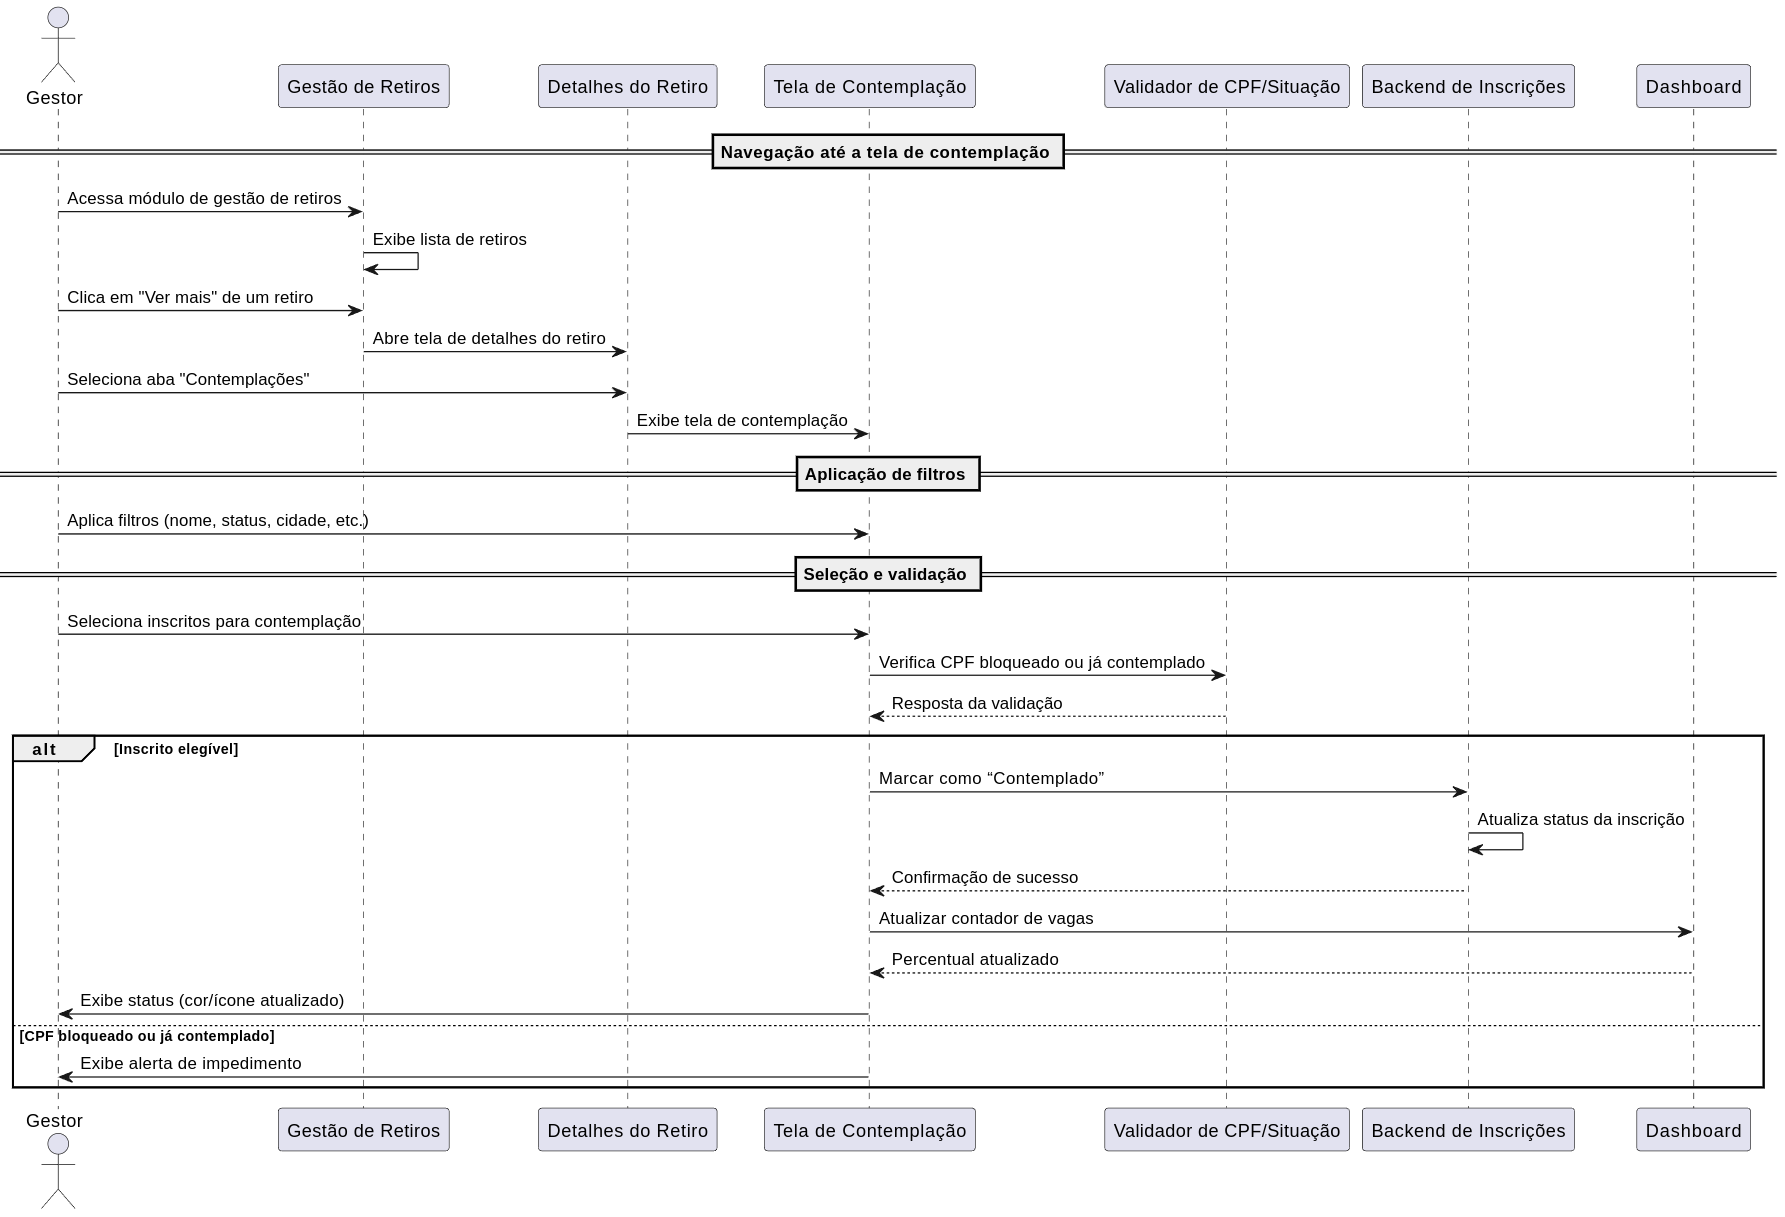
\includegraphics[width=0.9\textwidth]{images/diagramasdesequencias/participantContemplation.png}
    \caption{Diagrama de sequência para contemplação de participantes}
    \label{fig:participantContemplation}
\end{figure}

O processo se inicia quando o gestor acessa a área de gestão de retiros e, em seguida, a aba “Contemplações” de um retiro específico. Nessa tela, é possível aplicar filtros para facilitar a busca de participantes. Após selecionar os inscritos desejados, o sistema realiza uma verificação para validar se o CPF está bloqueado ou se o participante já foi contemplado.

Se o participante for elegível, o backend atualiza o status para “Contemplado” e o dashboard é atualizado para refletir o novo percentual de vagas ocupadas. O sistema então exibe o novo status visualmente ao gestor. Caso haja impedimentos, como CPF bloqueado ou contemplação anterior, o sistema alerta o gestor e impede a finalização da ação.


A Figura~\ref{fig:contemplationMessageSend} ilustra o fluxo realizado pelo gestor ao enviar mensagens personalizadas para os participantes contemplados, utilizando diferentes canais como WhatsApp e e-mail.

\begin{figure}[H]
    \centering
    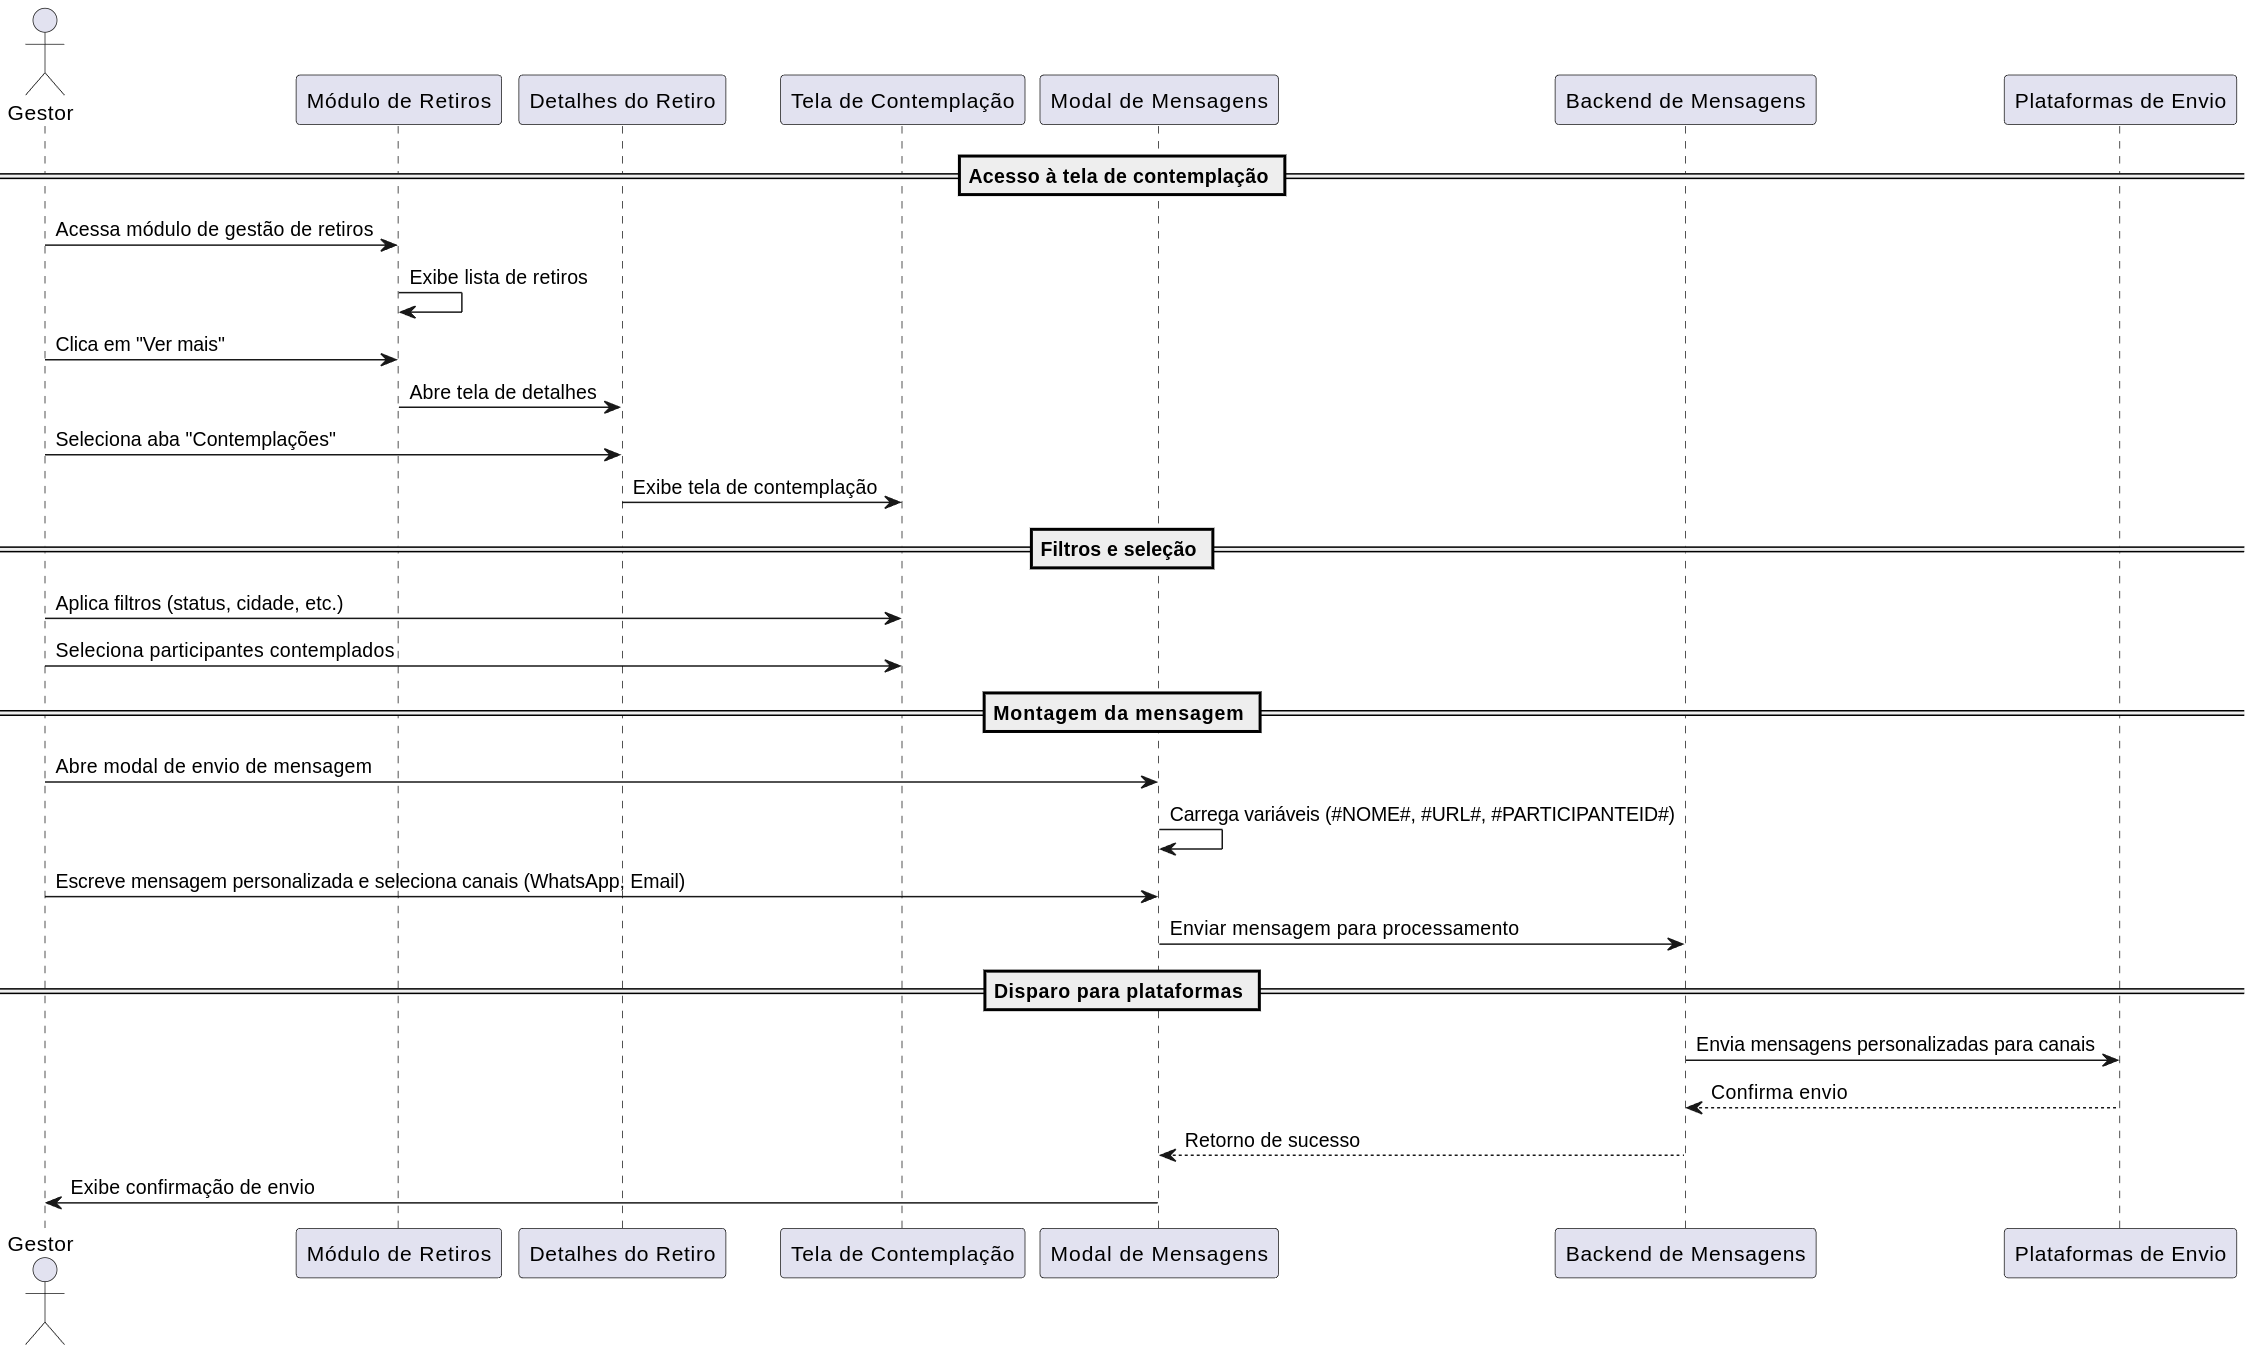
\includegraphics[width=0.9\textwidth]{images/diagramasdesequencias/manualContemplationMessage.png}
    \caption{Diagrama de sequência para envio de mensagem de contemplação}
    \label{fig:contemplationMessageSend}
\end{figure}

O fluxo se inicia com o gestor acessando o módulo de gestão de retiros e entrando na tela de detalhes de um retiro específico. Ao selecionar a aba “Contemplações”, é exibida a interface para aplicar filtros e selecionar os participantes que serão notificados.

Em seguida, o gestor abre o modal de mensagens, onde pode escrever o conteúdo da mensagem, utilizar variáveis como `\#NOME\#` e `\#URL\#`, e escolher os canais de envio. O backend de mensagens processa o conteúdo e o distribui para as plataformas responsáveis, como APIs de WhatsApp e serviços de e-mail. Após a confirmação do envio, o sistema exibe uma mensagem de sucesso ao gestor.

\subsection{Diagrama de Sequência – Processo de Pagamento Automatizado}

A Figura~\ref{fig:participantPaymentAuto} descreve o fluxo de pagamento automatizado realizado pelo participante contemplado, desde a escolha do método até a confirmação automática da transação via webhook.

\begin{figure}[H]
    \centering
    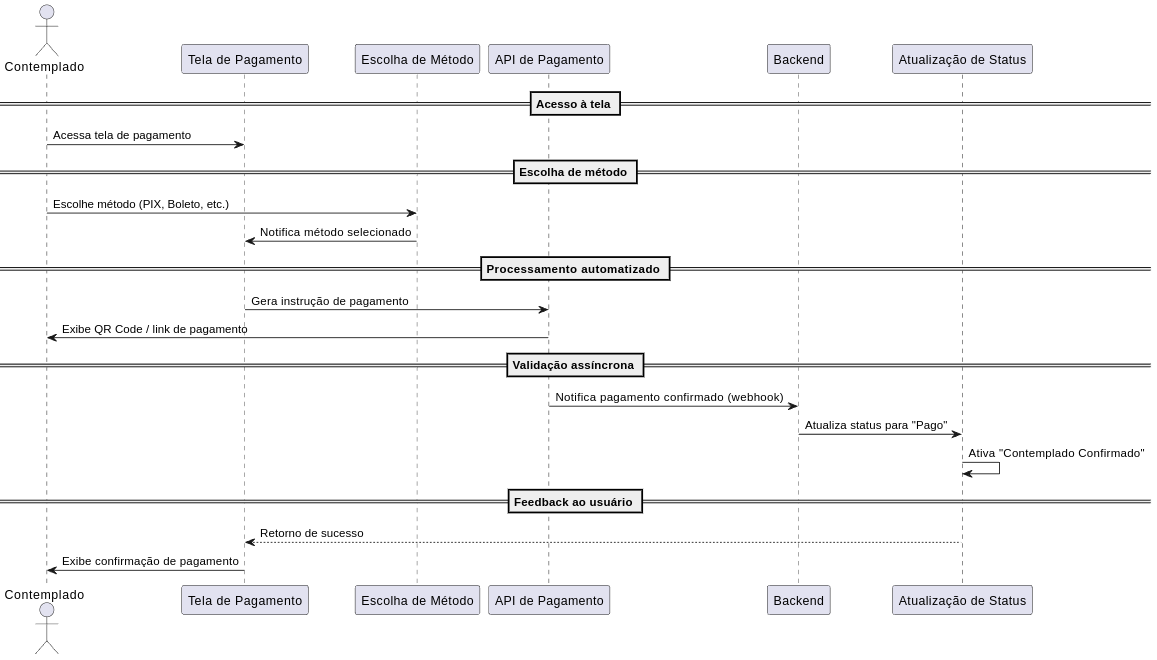
\includegraphics[width=0.9\textwidth]{images/diagramasdesequencias/participantPayment.png}
    \caption{Diagrama de sequência para processo de pagamento automatizado}
    \label{fig:participantPaymentAuto}
\end{figure}

O fluxo se inicia quando o participante contemplado acessa a tela de pagamento e seleciona o método desejado (como PIX ou boleto). O sistema, então, gera uma instrução de pagamento por meio de integração com uma API de pagamentos, que exibe ao usuário um QR Code ou link para realizar o pagamento.

Após o pagamento ser efetuado, a confirmação ocorre de forma assíncrona através de um webhook. A API de pagamentos notifica o backend, que atualiza o status da inscrição para “Pago” e ativa a confirmação da contemplação. Por fim, o sistema exibe ao usuário uma mensagem de confirmação com o status atualizado.

\subsection{Diagrama de Sequência – Composição Manual de Famílias}

A Figura~\ref{fig:familyManualComposition} descreve o fluxo de interação realizado pelo gestor ao compor manualmente as famílias do retiro, arrastando membros e validando regras de convivência, limite e diversidade.

\begin{figure}[H]
    \centering
    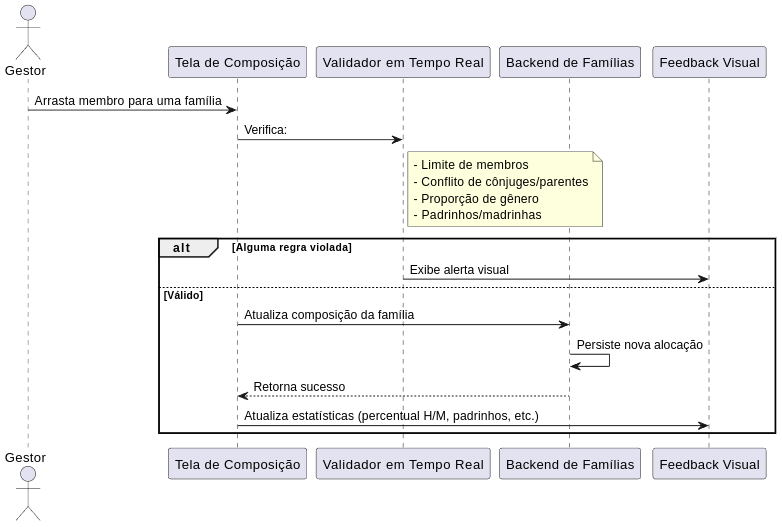
\includegraphics[width=0.9\textwidth]{images/diagramasdesequencias/familiyComposition.png}
    \caption{Diagrama de sequência para composição manual de famílias}
    \label{fig:familyManualComposition}
\end{figure}

O processo se inicia quando o gestor interage com a interface de composição e arrasta um membro para dentro de uma família. Imediatamente, o sistema realiza validações em tempo real para verificar se há violação de regras como o limite máximo de membros por família, conflito de parentesco, proporção de gênero e presença de padrinhos ou madrinhas.

Caso alguma regra seja violada, um alerta visual é exibido ao gestor. Caso contrário, a nova composição é enviada ao backend para persistência. O sistema então atualiza os dados e apresenta estatísticas atualizadas, como proporções de gênero e quantidade de padrinhos na família.

\subsection{Diagrama de Sequência – Sorteio Automático de Famílias}

A Figura~\ref{fig:familyAutoDraw} apresenta o fluxo realizado pelo gestor ao acionar a funcionalidade de sorteio automático para composição das famílias, com validação de regras e exibição de feedback visual.

\begin{figure}[H]
    \centering
    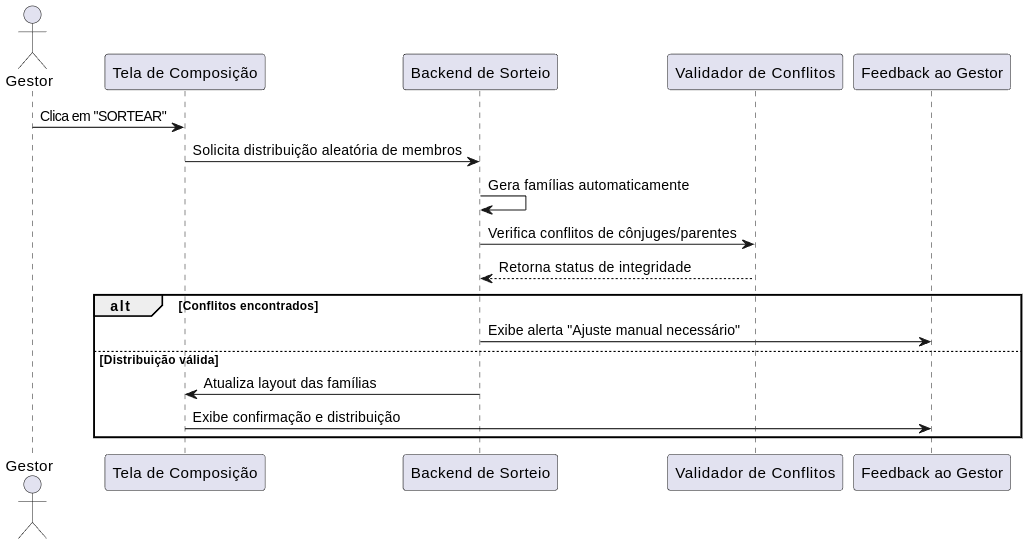
\includegraphics[width=0.9\textwidth]{images/diagramasdesequencias/familyDraw.png}
    \caption{Diagrama de sequência para sorteio automático de famílias}
    \label{fig:familyAutoDraw}
\end{figure}

O processo se inicia quando o gestor clica no botão “SORTEAR” na tela de composição de famílias. O sistema solicita ao backend a geração aleatória de famílias, que realiza a distribuição dos participantes conforme regras internas. Em seguida, um validador verifica possíveis conflitos, como membros da mesma família biológica sendo alocados juntos indevidamente.

Se forem encontrados conflitos, o sistema alerta o gestor para que ajustes manuais sejam realizados. Caso contrário, a nova composição é exibida automaticamente na interface, acompanhada de uma mensagem de sucesso e atualização visual da estrutura familiar.

\subsection{Diagrama de Sequência – Cadastro de Famílias}

A Figura~\ref{fig:familyCreate} apresenta o fluxo realizado pelo gestor ao cadastrar uma nova família no sistema, vinculando-a a um retiro específico.

\begin{figure}[H]
    \centering
    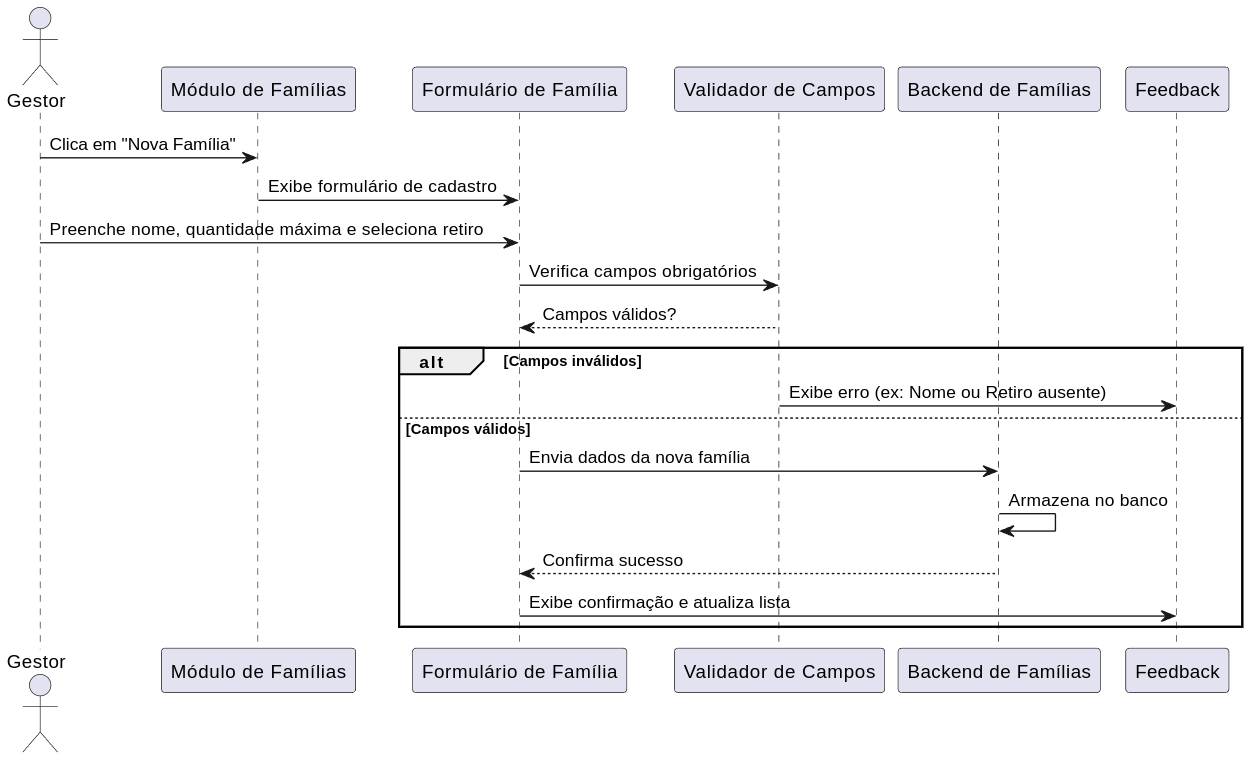
\includegraphics[width=0.9\textwidth]{images/diagramasdesequencias/familyRegister.png}
    \caption{Diagrama de sequência para cadastro de famílias}
    \label{fig:familyCreate}
\end{figure}

O processo tem início quando o gestor acessa o módulo de famílias e clica na opção “Nova Família”. Em seguida, o sistema exibe um formulário no qual o gestor deve preencher o nome da família, a quantidade máxima de membros e o retiro ao qual ela será vinculada.

Após o preenchimento, o sistema valida os campos obrigatórios. Se houver erros, como ausência do nome ou do retiro, uma mensagem de erro é exibida. Caso os dados estejam corretos, o backend realiza o armazenamento no banco de dados e retorna uma confirmação de sucesso. A interface é então atualizada, exibindo a nova família na lista.

\subsection{Diagrama de Sequência – Criação de Grupos de WhatsApp por Família}

A Figura~\ref{fig:familyWhatsappGroup} apresenta o fluxo realizado pelo gestor ao acionar a funcionalidade de criação automática de grupos de WhatsApp para as famílias cadastradas no retiro.

\begin{figure}[H]
    \centering
    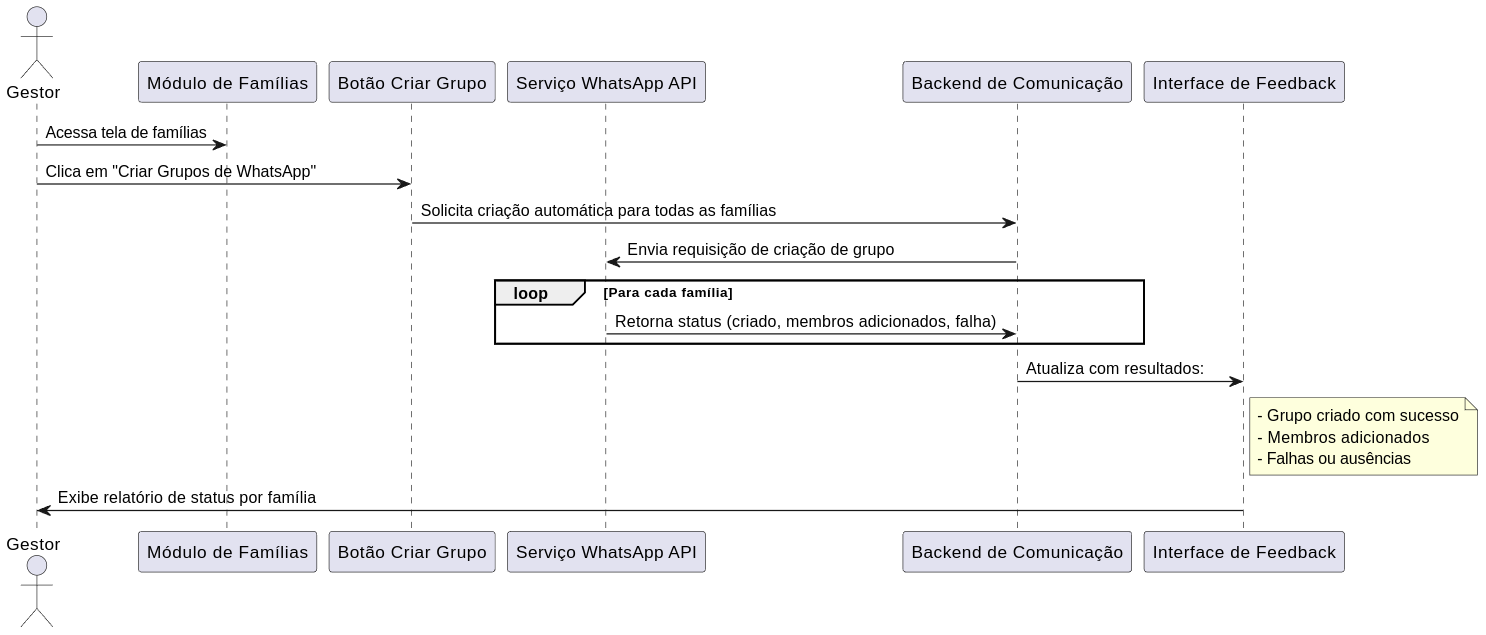
\includegraphics[width=0.9\textwidth]{images/diagramasdesequencias/familyWpGroup.png}
    \caption{Diagrama de sequência para criação de grupos de WhatsApp por família}
    \label{fig:familyWhatsappGroup}
\end{figure}

O processo é iniciado quando o gestor acessa a tela de famílias e clica no botão “Criar Grupos de WhatsApp”. O sistema então aciona o backend de comunicação, que se comunica com a API do WhatsApp para criar os grupos automaticamente, um para cada família registrada.

Durante o processo, o backend recebe o status individual de cada operação, como criação do grupo, adição dos membros e possíveis falhas. Ao final, um relatório de status é exibido ao gestor, informando os resultados para cada família — incluindo sucesso, falhas ou ausência de membros vinculados.

\subsection{Diagrama de Sequência – Atribuição de Funções na Equipe de Serviço}

A Figura~\ref{fig:teamRoleAssign} apresenta o fluxo realizado pelo gestor ao atribuir funções específicas (como Coordenador, Vice ou Membro) aos participantes de uma equipe de serviço.

\begin{figure}[H]
    \centering
    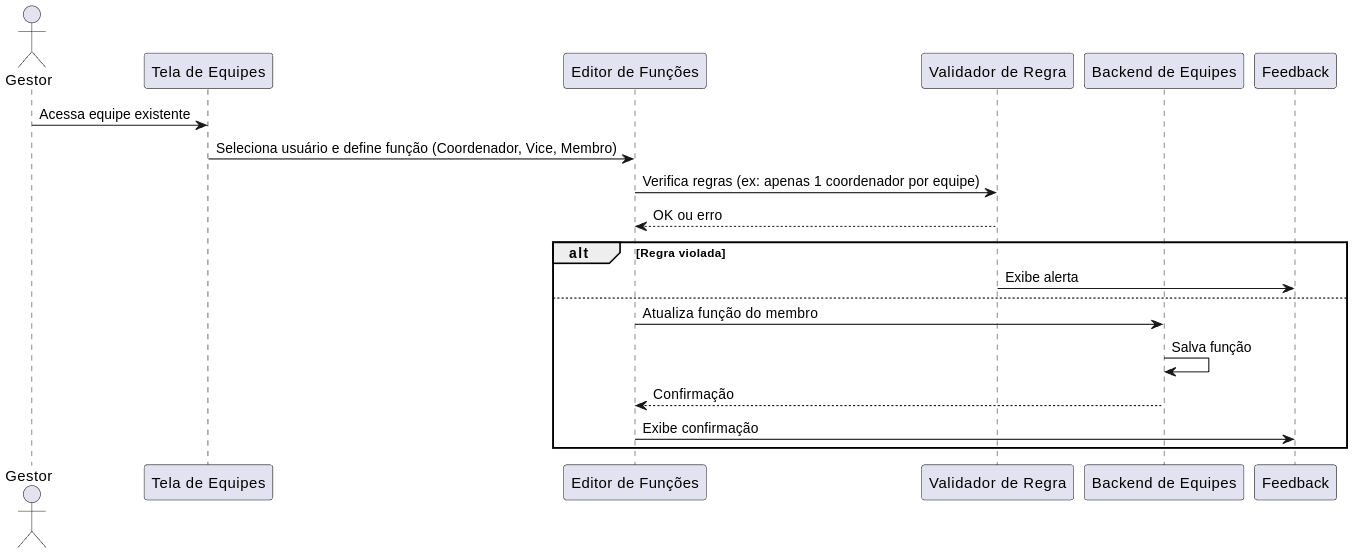
\includegraphics[width=0.9\textwidth]{images/diagramasdesequencias/teamAtribuition.png}
    \caption{Diagrama de sequência para atribuição de funções na equipe de serviço}
    \label{fig:teamRoleAssign}
\end{figure}

O processo se inicia quando o gestor acessa uma equipe existente na tela de equipes e seleciona um dos participantes para definir sua função. O sistema verifica se as regras específicas da composição da equipe estão sendo respeitadas, como a limitação de apenas um coordenador por equipe.

Se alguma regra for violada, é exibido um alerta visual com o motivo do impedimento. Caso contrário, a nova função é enviada ao backend para ser salva, e uma confirmação de sucesso é apresentada ao gestor.

\subsection{Diagrama de Sequência – Cadastro de Equipe de Serviço}

A Figura~\ref{fig:teamCreate} apresenta o fluxo realizado pelo gestor ao cadastrar uma nova equipe de serviço, utilizando um formulário manual ou com base em um modelo pré-cadastrado.

\begin{figure}[H]
    \centering
    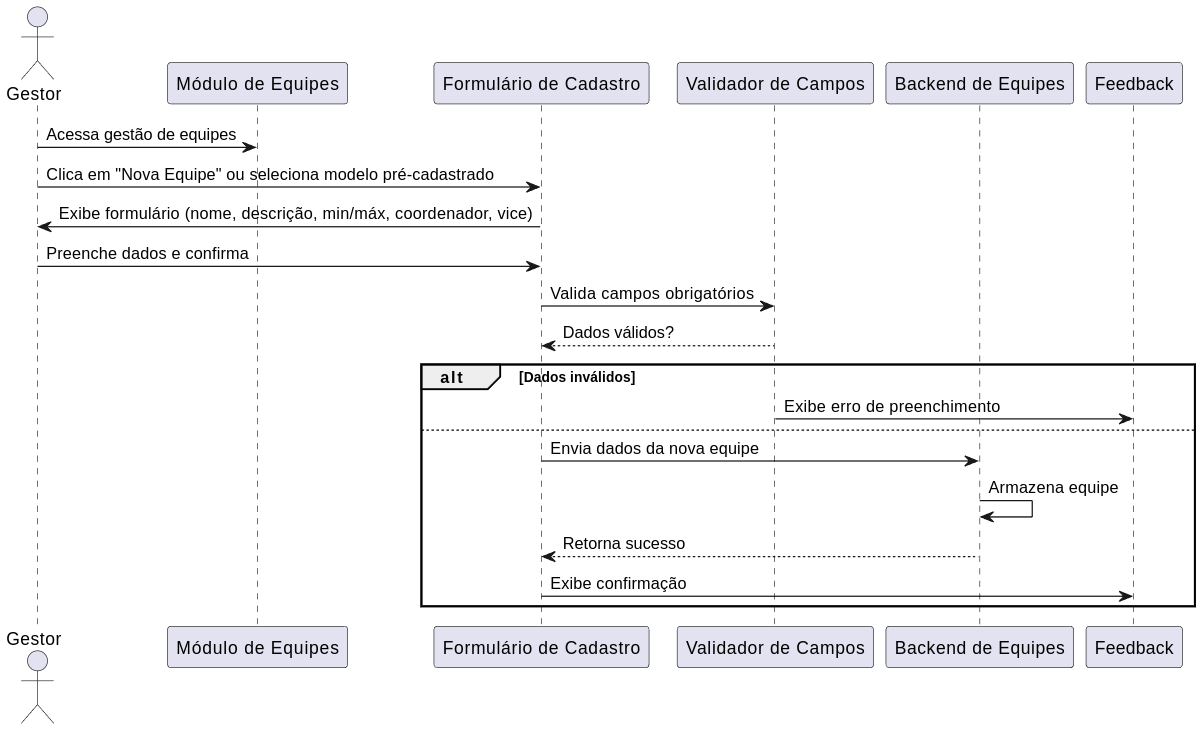
\includegraphics[width=0.9\textwidth]{images/diagramasdesequencias/teamCreate.png}
    \caption{Diagrama de sequência para cadastro de equipe de serviço}
    \label{fig:teamCreate}
\end{figure}

O processo tem início com o gestor acessando o módulo de equipes e clicando em “Nova Equipe” ou selecionando um modelo existente. O sistema apresenta um formulário para preenchimento de informações como nome, descrição, número mínimo e máximo de membros, e seleção de coordenador e vice.

Após o preenchimento, os campos obrigatórios são validados. Caso haja erros, o sistema exibe uma mensagem orientando a correção. Se os dados estiverem corretos, o backend realiza o armazenamento da equipe e retorna uma confirmação, que é então exibida ao gestor.

\subsection{Diagrama de Sequência – Distribuição de Membros nas Equipes}

A Figura~\ref{fig:teamDistribution} descreve o processo de movimentação de membros entre equipes de serviço, respeitando os limites máximos de alocação definidos para cada equipe.

\begin{figure}[H]
    \centering
    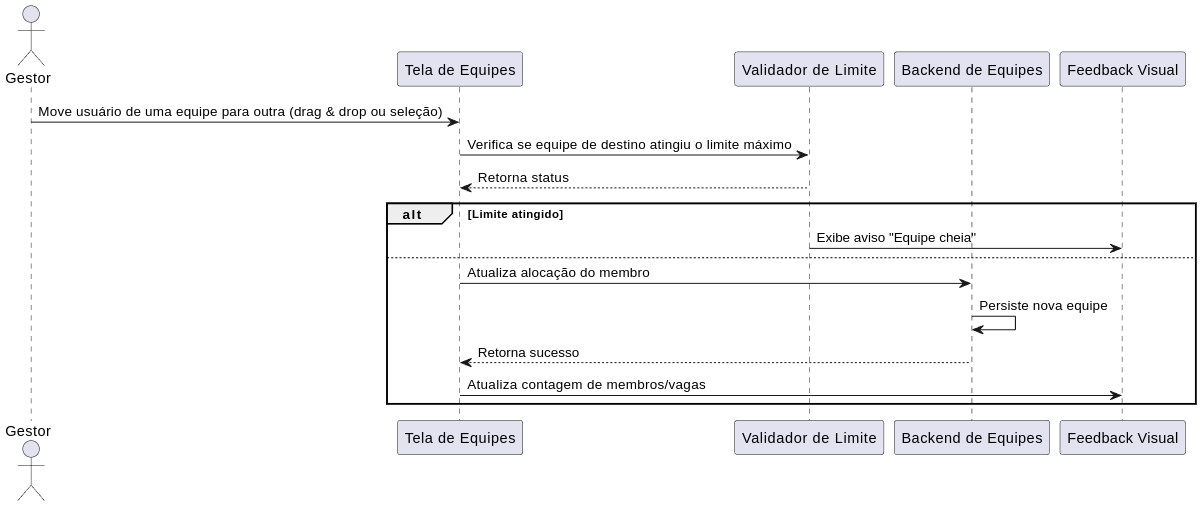
\includegraphics[width=0.9\textwidth]{images/diagramasdesequencias/teamDistribution.png}
    \caption{Diagrama de sequência para distribuição de membros nas equipes}
    \label{fig:teamDistribution}
\end{figure}

O fluxo se inicia quando o gestor interage com a tela de equipes e move um membro de uma equipe para outra, seja por arraste (drag \texttt{\&} drop) ou por seleção direta. O sistema valida se a equipe de destino ainda possui vagas disponíveis.

Caso o limite máximo de membros já tenha sido atingido, um aviso é exibido ao gestor informando que a equipe está cheia. Caso contrário, a nova alocação é enviada ao backend, que persiste a alteração e retorna uma confirmação. A interface é então atualizada com a nova contagem de membros e vagas disponíveis.

\subsection{Diagrama de Sequência – Cadastro de Barracas}

A Figura~\ref{fig:tentCreate} apresenta o fluxo de cadastro de barracas realizado pelo gestor, tanto de forma individual quanto por meio da funcionalidade de cadastro em lote.

\begin{figure}[H]
    \centering
    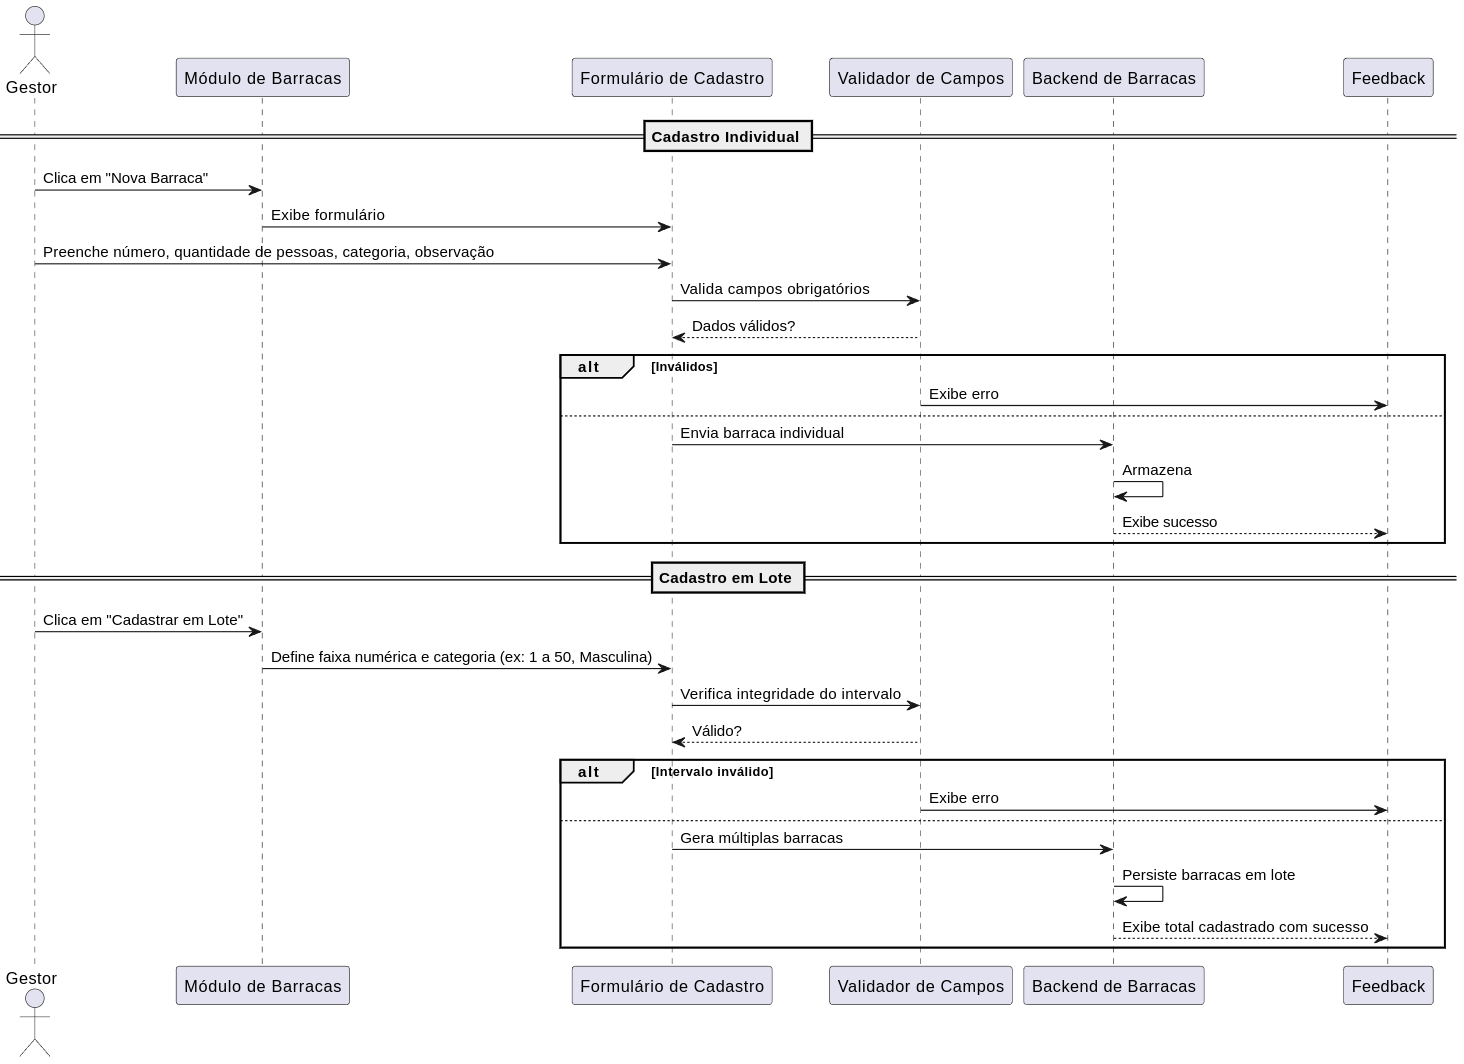
\includegraphics[width=0.9\textwidth]{images/diagramasdesequencias/tentCreation.png}
    \caption{Diagrama de sequência para cadastro de barracas}
    \label{fig:tentCreate}
\end{figure}

No modo de cadastro individual, o gestor clica em “Nova Barraca” e preenche informações como número, capacidade, categoria e observações. O sistema valida os campos obrigatórios e, se estiverem corretos, envia os dados para o backend, que realiza o armazenamento e retorna uma mensagem de sucesso.

No modo de cadastro em lote, o gestor informa uma faixa numérica (por exemplo, de 1 a 50) e a categoria das barracas. O sistema valida o intervalo e, se for válido, gera automaticamente as barracas correspondentes e realiza a persistência em lote. Ao final, uma mensagem de confirmação com o total de barracas cadastradas é exibida ao gestor.

\subsection{Diagrama de Sequência – Atribuição de Participante à Barraca}

A Figura~\ref{fig:tentAssign} descreve o fluxo realizado pelo gestor ao alocar manualmente um participante em uma barraca, verificando automaticamente a disponibilidade da mesma.

\begin{figure}[H]
    \centering
    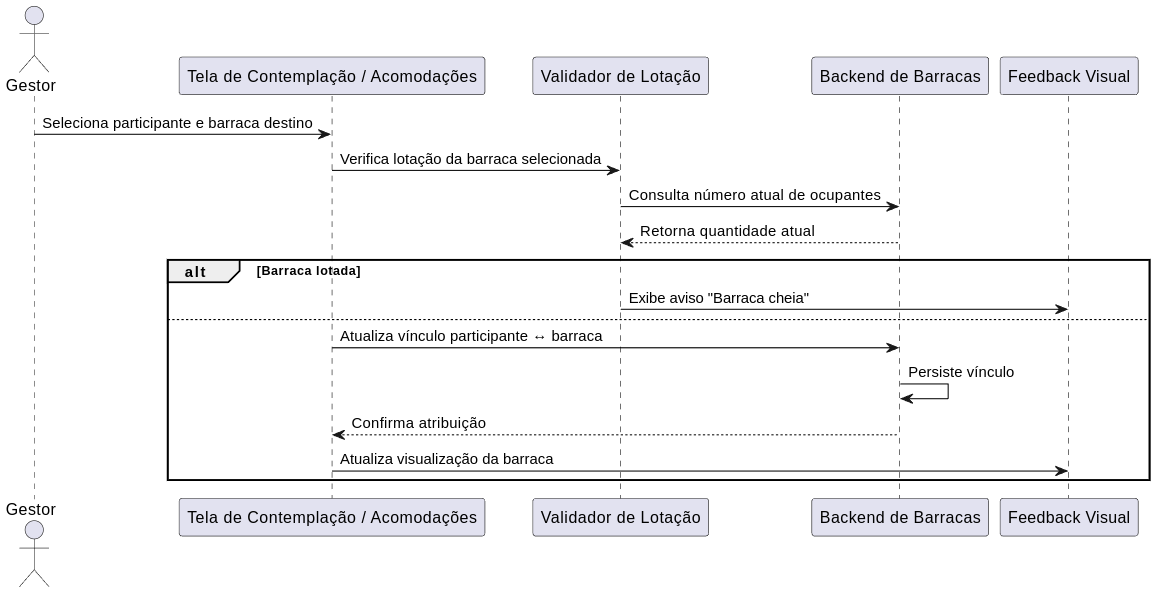
\includegraphics[width=0.9\textwidth]{images/diagramasdesequencias/tentaddParticipant.png}
    \caption{Diagrama de sequência para atribuição de participante à barraca}
    \label{fig:tentAssign}
\end{figure}

O fluxo se inicia quando o gestor seleciona um participante e escolhe uma barraca de destino na interface de acomodações. O sistema valida a lotação da barraca, consultando o backend para obter a quantidade atual de ocupantes.

Se a barraca já estiver cheia, o sistema exibe um aviso visual informando a indisponibilidade. Caso contrário, o vínculo entre participante e barraca é atualizado no backend e a interface é atualizada com a nova alocação, refletindo visualmente a ocupação da barraca.

\subsection{Diagrama de Sequência – Inscrição Pública}

A Figura~\ref{fig:publicInscription} apresenta o fluxo realizado por um visitante ao acessar o formulário público de inscrição para um retiro e realizar sua candidatura.

\begin{figure}[H]
    \centering
    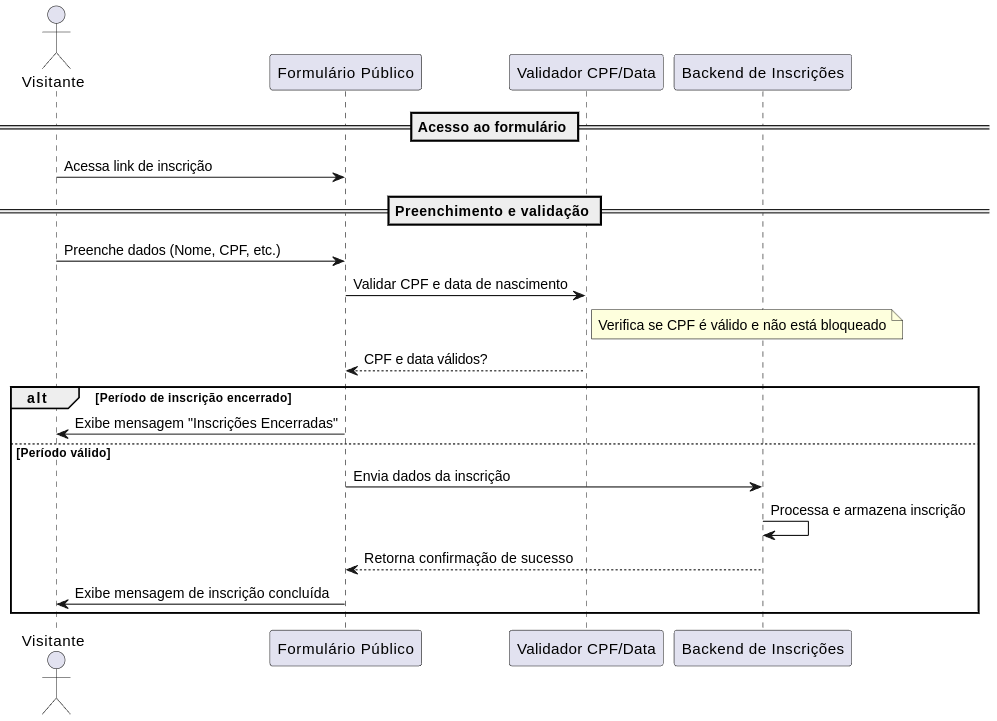
\includegraphics[width=0.9\textwidth]{images/diagramasdesequencias/participantFormSubscription.png}
    \caption{Diagrama de sequência para inscrição pública}
    \label{fig:publicInscription}
\end{figure}

O fluxo se inicia com o visitante acessando o link público de inscrição. Ao preencher os dados solicitados, como nome e CPF, o sistema realiza a validação do CPF e da data de nascimento, incluindo verificações contra bloqueios.

Caso o período de inscrições esteja encerrado, o sistema exibe uma mensagem apropriada. Se a inscrição for válida, os dados são enviados ao backend, que os processa e armazena. Por fim, uma confirmação de sucesso é exibida ao visitante.


\subsection{Diagrama de Sequência – Recebimento da Mensagem e Acesso ao Sistema}

A Figura~\ref{fig:participantAccess} apresenta o fluxo realizado pelo participante contemplado ao receber a mensagem de confirmação e acessar o sistema por meio de um link personalizado.

\begin{figure}[H]
    \centering
    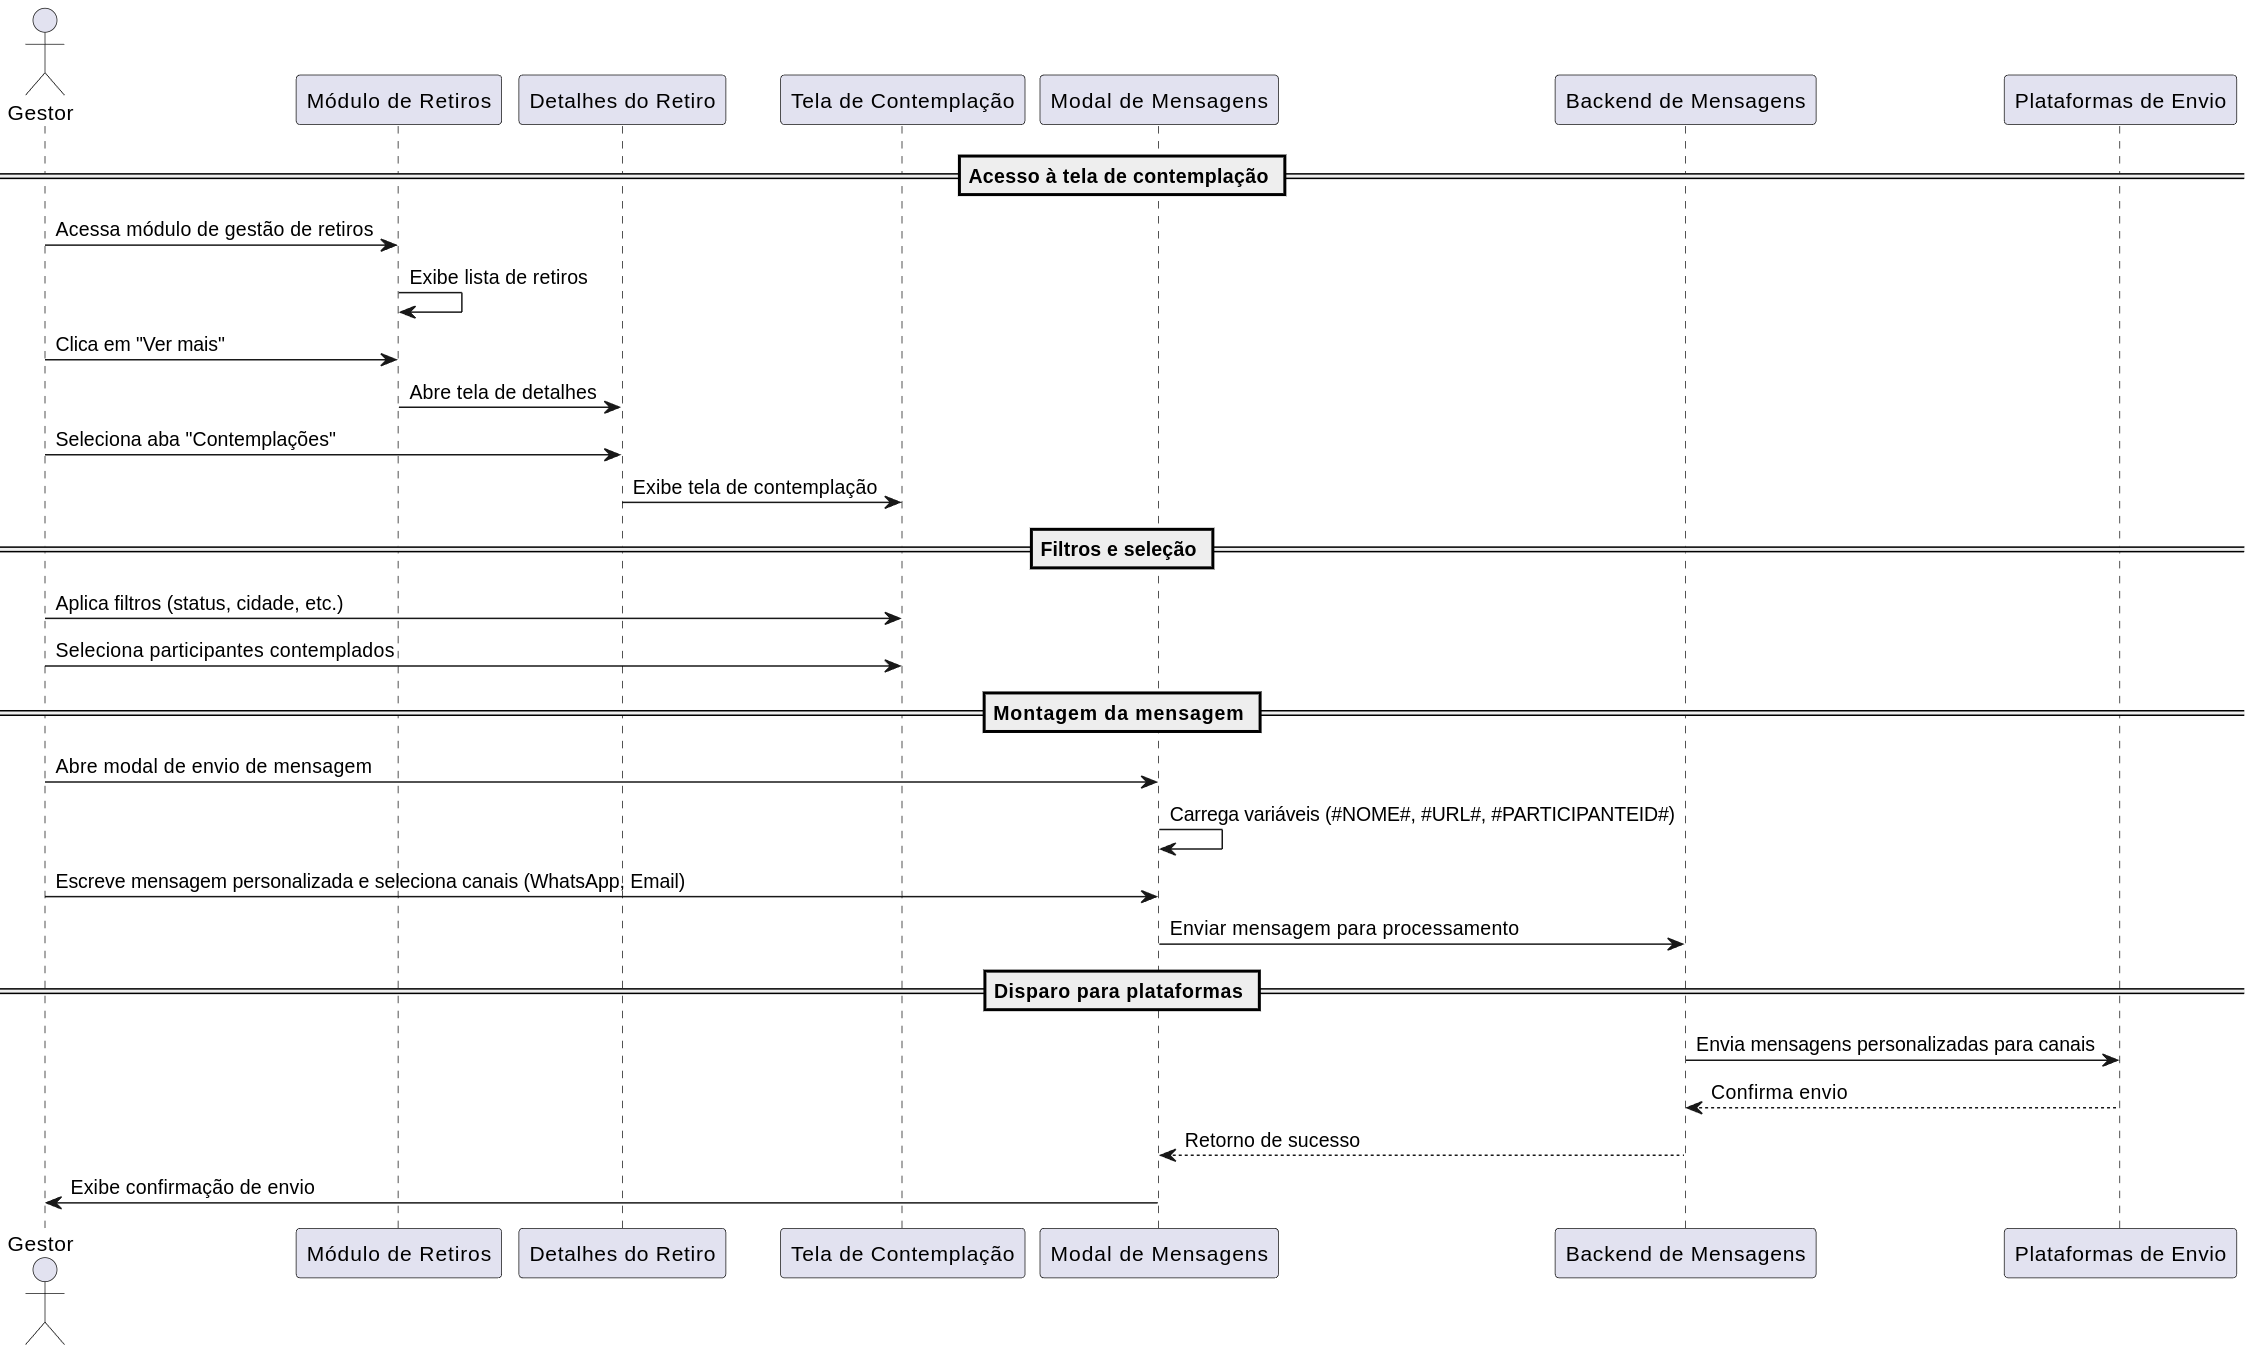
\includegraphics[width=0.9\textwidth]{images/diagramasdesequencias/manualContemplationMessage.png}
    \caption{Diagrama de sequência para recebimento da mensagem e acesso ao sistema}
    \label{fig:participantAccess}
\end{figure}

O fluxo se inicia com o envio da mensagem contendo o link de acesso individualizado, que é recebido pelo participante contemplado. Ao clicar nesse link, ele é redirecionado para a tela de cadastro, já contendo seu identificador (`ContempladoID`) de forma embutida.

Na tela de cadastro, o participante preenche os dados solicitados e confirma. O backend valida e armazena as informações, retornando sucesso. Em seguida, o sistema redireciona automaticamente o usuário para a tela inicial, que contém seus dados pessoais, informações sobre o retiro para o qual foi contemplado e a área de pagamento.

\subsection{Diagrama de Sequência – Processo de Pagamento Automatizado (Versão Atualizada)}

A Figura~\ref{fig:participantPaymentAutoV2} descreve o fluxo realizado pelo participante ao efetuar um pagamento via sistema integrado, com atualização imediata do status para "Pagamento Pendente" após a escolha do método, e confirmação automática via webhook.

\begin{figure}[H]
    \centering
    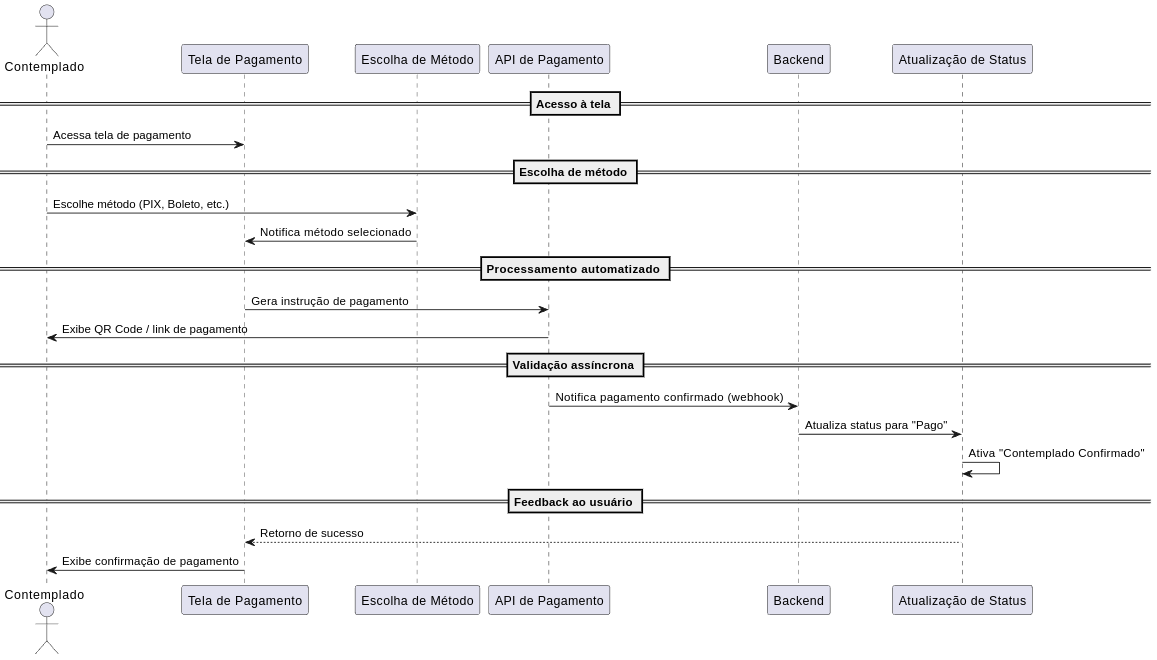
\includegraphics[width=0.9\textwidth]{images/diagramasdesequencias/participantPayment.png}
    \caption{Diagrama de sequência para processo de pagamento automatizado com status pendente}
    \label{fig:participantPaymentAutoV2}
\end{figure}

O fluxo se inicia com o acesso do participante à tela de pagamento, onde ele escolhe o método desejado (como PIX ou Boleto). Após a seleção, o sistema registra o status como “Pagamento Pendente” e gera a instrução de pagamento via integração com a API de pagamentos, que fornece um QR Code ou link para efetivação.

O pagamento é confirmado de forma assíncrona, por meio de um webhook da API de pagamentos para o backend. Após o recebimento dessa confirmação, o status da inscrição é atualizado para “Pago” e o sistema marca o participante como “Confirmado”. Por fim, o participante recebe o feedback de sucesso com a confirmação visual da operação.

\subsection{Diagrama de Sequência – Geração de Relatório}

A Figura~\ref{fig:reportGeneration} apresenta o fluxo realizado pelo gestor ao gerar relatórios com base em filtros definidos, permitindo tanto a visualização em tela quanto a exportação para PDF ou CSV.

\begin{figure}[H]
    \centering
    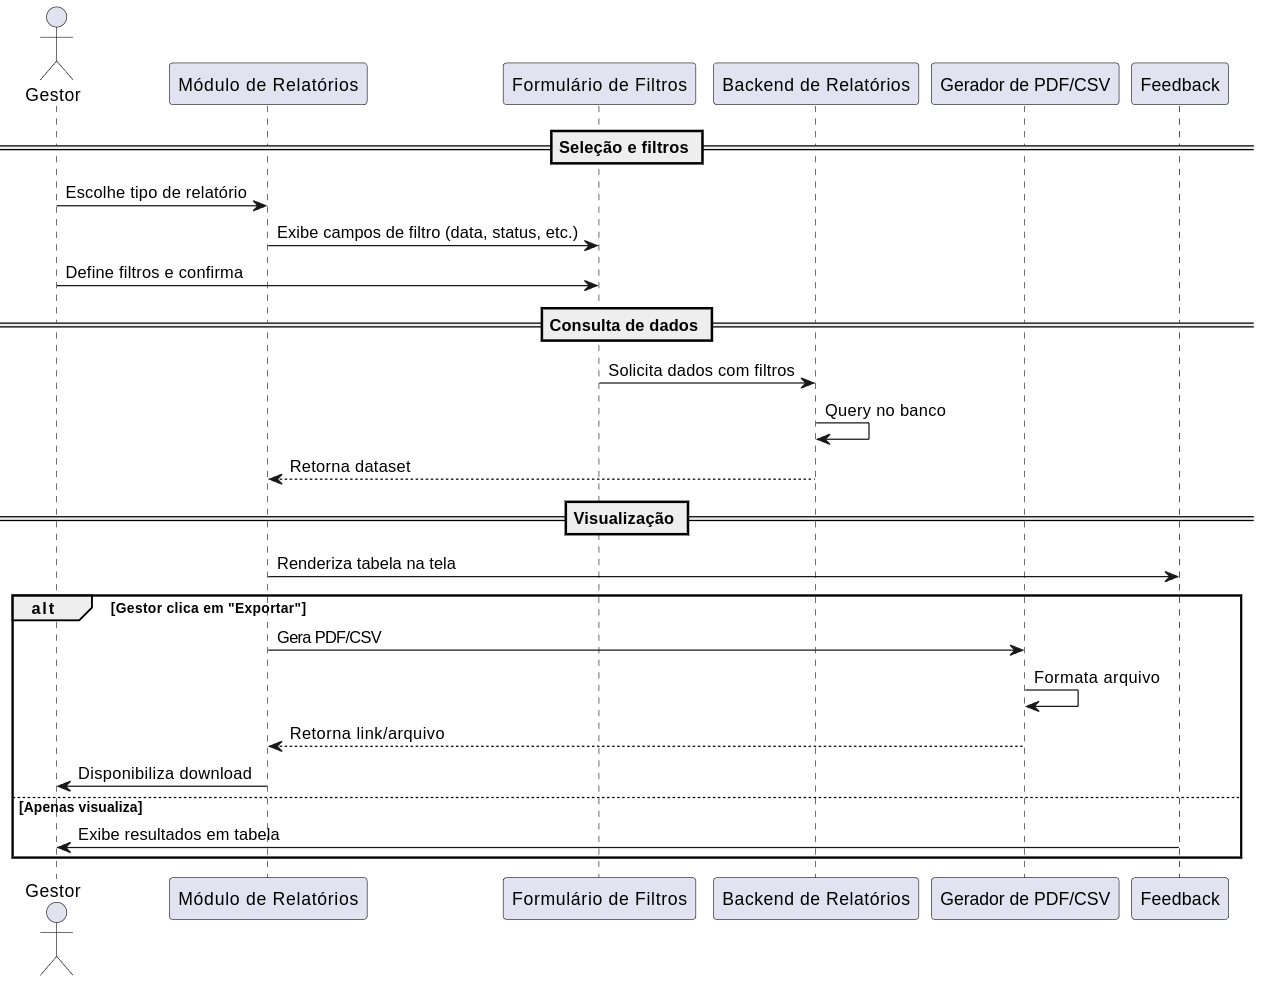
\includegraphics[width=0.9\textwidth]{images/diagramasdesequencias/report.png}
    \caption{Diagrama de sequência para geração de relatório}
    \label{fig:reportGeneration}
\end{figure}

O processo inicia-se quando o gestor acessa o módulo de relatórios e seleciona o tipo de relatório desejado. Em seguida, o sistema exibe os filtros disponíveis, como data, status ou outras informações relevantes. Após configurar os filtros, o sistema consulta o backend, que realiza uma busca no banco de dados e retorna os dados correspondentes.

Esses dados são renderizados em uma tabela visual na interface. Caso o gestor opte por exportar os resultados, o sistema aciona o gerador de arquivos (PDF ou CSV), que formata e retorna o arquivo para download. Se não houver exportação, a visualização permanece apenas em tela.

\subsection{Diagrama de Sequência – Notificações}

A Figura~\ref{fig:notificationFlow} apresenta o fluxo de funcionamento do sistema de notificações, desde o carregamento das mensagens até a navegação para o conteúdo relacionado à notificação selecionada.

\begin{figure}[H]
    \centering
    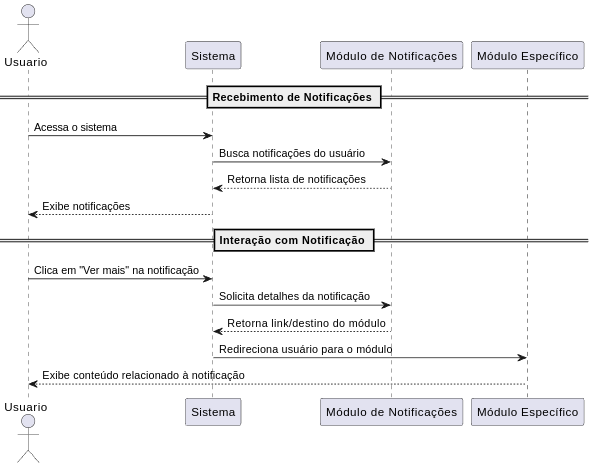
\includegraphics[width=0.9\textwidth]{images/diagramasdesequencias/notification.png}
    \caption{Diagrama de sequência para recebimento e interação com notificações}
    \label{fig:notificationFlow}
\end{figure}

O fluxo se inicia quando o usuário acessa o sistema. Neste momento, o sistema solicita ao módulo de notificações as mensagens destinadas ao usuário. A lista de notificações é retornada e exibida de forma resumida na interface.

Ao interagir com uma notificação (clicando em “Ver mais”), o sistema solicita ao módulo de notificações os detalhes da mensagem, incluindo o destino associado. O usuário é então redirecionado para o módulo correspondente, onde poderá visualizar o conteúdo relacionado à notificação.
